\documentclass[12pt,a4paper]{article}

% === PACKAGES ===
\usepackage[utf8]{inputenc}
\usepackage[T5]{fontenc}
\usepackage{scrextend}
\changefontsizes{13pt}
\usepackage{amsmath, amssymb, amsfonts}
\usepackage{graphicx}
\usepackage{booktabs}
\usepackage{caption}
\usepackage{subcaption}
\usepackage{geometry}
\usepackage{hyperref}
\usepackage{cite}
\usepackage{enumitem}
\usepackage{float}
\usepackage{algorithm}
\usepackage{algpseudocode}
\usepackage{bm}
\usepackage{multirow}
\usepackage{arydshln}
\usepackage{indentfirst}
\usepackage{titlesec}
\usepackage{fancyhdr}
\usepackage{tikz}
\usetikzlibrary{arrows.meta, positioning, shapes.geometric, calc, decorations.pathreplacing, patterns}
\usepackage{pgfplots}
\pgfplotsset{compat=1.18}

% === GEOMETRY (chuẩn HUST) ===
\geometry{right=2cm, left=3cm, top=2cm, bottom=2.5cm}
\graphicspath{{figures/}}

% === LINE SPACING ===
\renewcommand{\baselinestretch}{1.2}

% === HEADING STYLES ===
\titleformat{\section}[block]{\centering\bfseries\fontsize{16}{19}\selectfont}{}{0em}{}
\titleformat{\subsection}[block]{\bfseries\fontsize{14}{17}\selectfont}{}{0em}{}
\titleformat{\subsubsection}[block]{\bfseries\fontsize{13}{16}\selectfont}{}{0em}{}

% === FIGURE/TABLE NUMBERING ===
\makeatletter
\newcommand{\chapternum}{0}
\newcommand{\setchapter}[1]{%
  \renewcommand{\chapternum}{#1}%
  \setcounter{figure}{0}%
  \setcounter{table}{0}%
  \setcounter{equation}{0}%
  \renewcommand{\thefigure}{\chapternum.\arabic{figure}}%
  \renewcommand{\thetable}{\chapternum.\arabic{table}}%
  \renewcommand{\theequation}{\chapternum.\arabic{equation}}%
}
\makeatother

% === MATH COMMANDS ===
\newcommand{\R}{\mathbb{R}}
\newcommand{\T}{\mathsf{T}}
\DeclareMathOperator{\diag}{diag}
\DeclareMathOperator{\sign}{sign}
\DeclareMathOperator{\rank}{rank}

% ================================================================
\begin{document}

% ================================================================
% BÌA LUẬN VĂN
% ================================================================
\begin{titlepage}
\thispagestyle{empty}
\begin{tikzpicture}[overlay,remember picture]
\draw [line width=3pt]
    ($ (current page.north west) + (3.2cm,-2.2cm) $)
    rectangle
    ($ (current page.south east) + (-2.2cm,2.7cm) $);
\draw [line width=0.5pt]
    ($ (current page.north west) + (3.3cm,-2.3cm) $)
    rectangle
    ($ (current page.south east) + (-2.3cm,2.8cm) $);
\end{tikzpicture}
\begin{center}

\vspace*{0.3cm}
{\fontsize{15}{18}\selectfont ĐẠI HỌC BÁCH KHOA HÀ NỘI}\\[4pt]
{\fontsize{13}{16}\selectfont\bfseries TRƯỜNG ĐIỆN -- ĐIỆN TỬ}\\[0.6cm]


\includegraphics[width=0.13\textwidth]{logoBK.png}\\[0.6cm]

{\fontsize{20}{24}\selectfont\bfseries LUẬN VĂN THẠC SĨ}\\[1.0cm]

{\fontsize{15}{18}\selectfont\bfseries ĐIỀU KHIỂN TỐI ƯU THÍCH NGHI DỰA TRÊN\\[6pt]
QUY HOẠCH ĐỘNG HỘI TỤ CỐ ĐỊNH THỜI GIAN\\[6pt]
CHO ROBOT DI ĐỘNG HAI BÁNH}\\[1.5cm]

\begin{tabular}{rl}
{\fontsize{14}{16}\selectfont \textbf{Học viên:}} & {\fontsize{14}{16}\selectfont \textbf{NGUYỄN THÀNH TRUNG}} \\[4pt]
{\fontsize{13}{15}\selectfont \textit{Email:}} & {\fontsize{13}{15}\selectfont trung.nt242245m@sis.hust.edu.vn} \\[4pt]
{\fontsize{13}{15}\selectfont \textbf{Ngành:}} & {\fontsize{13}{15}\selectfont Kỹ thuật Điều khiển và Tự động hóa} \\
\end{tabular}

\vspace{1.5cm}

\begin{tabular}{ll}
{\fontsize{14}{16}\selectfont Giáo viên hướng dẫn:} & {\fontsize{14}{16}\selectfont PGS.TS. Nguyễn Hoài Nam}
\end{tabular}

\vfill

{\fontsize{14}{17}\selectfont Hà Nội, 06/2026}

\end{center}
\end{titlepage}

% ================================================================
\newpage
\tableofcontents
\newpage

% ================================================================
% CHƯƠNG 1: GIỚI THIỆU
% ================================================================
\setchapter{1}
\section*{CHƯƠNG 1: GIỚI THIỆU}
\addcontentsline{toc}{section}{CHƯƠNG 1: GIỚI THIỆU}

\subsection*{1.1\quad Tổng quan về robot di động bánh xe}
\addcontentsline{toc}{subsection}{1.1\quad Tổng quan về robot di động bánh xe}

Robot di động bánh xe (Wheeled Mobile Robot -- WMR) là một trong những nền tảng phổ biến nhất trong lĩnh vực robot học, được ứng dụng rộng rãi trong nhiều ngành công nghiệp và đời sống. Trong các nhà máy sản xuất, robot di động được sử dụng để vận chuyển hàng hóa tự động (AGV -- Automated Guided Vehicle), giảm thiểu sức lao động con người và tăng hiệu suất sản xuất. Trong lĩnh vực dịch vụ, robot di động phục vụ trong bệnh viện, nhà hàng, và các tòa nhà thông minh. Trong nghiên cứu khoa học, WMR là nền tảng thí nghiệm lý tưởng cho các thuật toán điều khiển, lập kế hoạch đường đi, và trí tuệ nhân tạo.

\begin{figure}[H]
\centering

\includegraphics[width=0.35\textwidth]{agv_example.png}
\caption{Robot AGV vận chuyển hàng hóa tự động trong nhà máy}
\label{fig:agv_example}
\end{figure}

Robot di động bánh xe vi sai (differential-drive WMR) là cấu hình đơn giản và phổ biến nhất, gồm hai bánh chủ động độc lập và một hoặc nhiều bánh đỡ. Mặc dù cấu trúc cơ khí đơn giản, việc điều khiển WMR vi sai đặt ra nhiều thách thức lý thuyết đáng kể:

\begin{itemize}
    \item \textbf{Ràng buộc phi holonomic (nonholonomic constraint):} Robot không thể dịch chuyển ngang (perpendicular to its heading direction). Ràng buộc này biểu hiện dưới dạng $\dot{x}\sin\theta - \dot{y}\cos\theta = 0$, nghĩa là vector vận tốc của robot luôn hướng theo trục dọc của thân xe. Hệ quả là không gian trạng thái có thể đạt được (reachable set) bị giới hạn tại mỗi thời điểm, khiến các phương pháp điều khiển tuyến tính thông thường không áp dụng trực tiếp được.

    \item \textbf{Tính phi tuyến mạnh:} Mô hình động học (kinematic model) của WMR chứa các hàm lượng giác $\cos\theta$, $\sin\theta$ phụ thuộc vào góc hướng, dẫn đến hệ phương trình phi tuyến bản chất. Khi kết hợp thêm mô hình động lực học (dynamic model) với ma sát, quán tính, và bão hòa mô-men, độ phức tạp tăng lên đáng kể.

    \item \textbf{Bất định mô hình và nhiễu ngoài:} Trong thực tế, các tham số vật lý như khối lượng, mô-men quán tính, và hệ số ma sát không được biết chính xác. Ngoài ra, robot còn chịu tác động của nhiễu ngoài như mặt đường gồ ghề, gió, và tải trọng thay đổi.
\end{itemize}

Những thách thức trên đòi hỏi các phương pháp điều khiển tiên tiến, có khả năng xử lý phi tuyến, thích nghi với bất định, và đạt hiệu năng tối ưu.

\subsection*{1.2\quad Bài toán bám quỹ đạo và tối ưu hóa năng lượng}
\addcontentsline{toc}{subsection}{1.2\quad Bài toán bám quỹ đạo và tối ưu hóa năng lượng}

Bài toán bám quỹ đạo (trajectory tracking) yêu cầu robot di động đi theo một quỹ đạo tham chiếu $q_r(t) = [x_r(t), y_r(t), \theta_r(t)]^\T$ được xác định trước, sao cho sai số bám $z(t) = q_r(t) - q(t)$ hội tụ về không theo thời gian. Đây là bài toán cơ bản và quan trọng nhất trong điều khiển robot di động.

Tuy nhiên, trong nhiều ứng dụng thực tế, chỉ đạt được sai số bám nhỏ là chưa đủ. Robot cần hoạt động trong thời gian dài với nguồn năng lượng hữu hạn (pin), do đó việc \textbf{tối ưu hóa năng lượng} tiêu thụ đồng thời với việc duy trì chất lượng bám quỹ đạo trở nên thiết yếu. Bài toán được hình thức hóa thông qua hàm chi phí (cost function):
\begin{equation}\label{eq:cost_intro}
    J = \int_0^\infty \big( z^\T Q\, z + u_o^\T R\, u_o \big)\, dt
\end{equation}
trong đó $Q \geq 0$ là ma trận trọng số trạng thái (phạt sai số bám), $R > 0$ là ma trận trọng số điều khiển (phạt năng lượng tiêu thụ), và $u_o$ là tín hiệu điều khiển phản hồi (feedback control).

Hàm chi phí (\ref{eq:cost_intro}) thể hiện sự \textbf{đánh đổi (trade-off)} giữa hai mục tiêu mâu thuẫn: (i) bám quỹ đạo chính xác (giảm $z^\T Q z$), đòi hỏi tín hiệu điều khiển mạnh; và (ii) tiết kiệm năng lượng (giảm $u_o^\T R u_o$), đòi hỏi tín hiệu điều khiển nhỏ. Tỉ số $Q/R$ quyết định sự ưu tiên: $Q/R$ lớn ưu tiên bám chính xác, $Q/R$ nhỏ ưu tiên tiết kiệm năng lượng.

Bộ điều khiển tối ưu $u_o^*$ là nghiệm cực tiểu hóa $J$, thỏa mãn phương trình Hamilton-Jacobi-Bellman (HJB) -- một phương trình đạo hàm riêng phi tuyến nói chung không giải được bằng phương pháp giải tích, đặc biệt với hệ phi tuyến như WMR.

\subsection*{1.3\quad Các phương pháp điều khiển hiện nay và hạn chế}
\addcontentsline{toc}{subsection}{1.3\quad Các phương pháp điều khiển hiện nay và hạn chế}

\textbf{Backstepping (Kanayama et al. \cite{Kanayama1990}):} Phương pháp kinh điển cho WMR, thiết kế luật điều khiển đệ quy dựa trên hàm Lyapunov. Ưu điểm: đơn giản, hiệu quả cao khi mô hình chính xác. Hạn chế: (i) hội tụ tiệm cận (asymptotic), sai số giảm dần nhưng không triệt tiêu trong thời gian hữu hạn; (ii) không tối ưu năng lượng -- không tồn tại cơ chế cực tiểu hóa hàm chi phí; (iii) phụ thuộc mô hình, hiệu năng giảm khi có bất định.

\textbf{Sliding Mode Control (SMC):} Điều khiển trượt có khả năng kháng nhiễu (robustness) xuất sắc nhờ cơ chế chuyển mạch trên mặt trượt. Tuy nhiên: (i) hiện tượng chattering (dao động tần số cao quanh mặt trượt) gây hao mòn cơ cấu chấp hành; (ii) tiêu tốn năng lượng lớn do reaching law liên tục duy trì tín hiệu điều khiển mạnh; (iii) hàm chi phí $J$ rất cao, đặc biệt trên mô hình đầy đủ.

\textbf{ADP Actor-Critic (Vamvoudakis \& Lewis \cite{Vamvoudakis2010}):} Sử dụng hai mạng nơ-ron (Actor và Critic) để xấp xỉ nghiệm phương trình HJB. Ưu điểm: đạt được điều khiển gần tối ưu, thích nghi trực tuyến. Hạn chế: (i) yêu cầu tín hiệu kích thích liên tục (Persistence of Excitation -- PE) để đảm bảo hội tụ, mâu thuẫn với mục tiêu bám quỹ đạo; (ii) hai mạng riêng biệt làm tăng số lượng siêu tham số và phức tạp thiết kế; (iii) nhạy cảm với điều kiện khởi tạo (warm start).

\textbf{Điều khiển thời gian hữu hạn (Finite-time control):} Đảm bảo sai số hội tụ về không trong thời gian hữu hạn $T_f$. Tuy nhiên, $T_f$ phụ thuộc vào điều kiện đầu -- sai số ban đầu càng lớn thì thời gian hội tụ càng lâu, không có cận trên cố định cho mọi điều kiện đầu.

\subsection*{1.4\quad Đề xuất hướng tiếp cận}
\addcontentsline{toc}{subsection}{1.4\quad Đề xuất hướng tiếp cận}

Gần đây, Wang et al. \cite{Wang2025} đề xuất phương pháp ADP Fixed-time Optimal Control, kết hợp Quy hoạch động xấp xỉ (ADP) với ổn định cố định thời gian (Fixed-time stability, Polyakov \cite{Polyakov2012}). Phương pháp này đảm bảo sai số bám hội tụ trong thời gian xác định $T_f$ \textbf{độc lập với điều kiện ban đầu}, đồng thời đạt điều khiển gần tối ưu.

Tuy nhiên, Wang et al. chỉ xét \textbf{mô hình động học thuần túy} (kinematic model, 3 trạng thái $[x, y, \theta]$), bỏ qua hoàn toàn động lực học robot (quán tính, ma sát, giới hạn mô-men). Trong thực tế, sự hiện diện của động lực học là không thể tránh khỏi và ảnh hưởng đáng kể đến hiệu năng điều khiển.

\textbf{Đóng góp chính của luận văn:}
\begin{enumerate}
    \item \textbf{Mở rộng ADP Fixed-time sang kiến trúc hai vòng (dual-loop):} Vòng ngoài sử dụng ADP Fixed-time (phần kinematic), vòng trong sử dụng Dynamic Backstepping (phần dynamic, Fierro \& Lewis \cite{Fierro1997}), hoạt động trên mô hình đầy đủ 5 trạng thái $[x, y, \theta, v, \omega]$ với ma sát và nhiễu.

    \item \textbf{Điều chỉnh tham số robust cho kiến trúc hai vòng:} Phát hiện rằng các tham số robust trong Wang et al. (thiết kế cho kinematic-only) gây phát tán khi áp dụng trên dual-loop, và đề xuất phương pháp giảm gains 3--5 lần cùng cơ chế giới hạn (clamp) tín hiệu phản hồi.

    \item \textbf{So sánh toàn diện 5 phương pháp} trên mô hình đầy đủ: Backstepping, Actor-Critic ADP, SMC, Critic-only Concurrent Learning, và ADP Fixed-time, trên 3 loại quỹ đạo và nhiều điều kiện vận hành.

    \item \textbf{Phân tích robustness:} Đánh giá khả năng kháng bất định khối lượng và nhiễu ngoài của các phương pháp.
\end{enumerate}

\subsection*{1.5\quad Cấu trúc luận văn}
\addcontentsline{toc}{subsection}{1.5\quad Cấu trúc luận văn}

Luận văn được tổ chức thành 6 chương:

\begin{itemize}[nosep]
    \item \textbf{Chương 1: Giới thiệu} -- Trình bày bối cảnh, bài toán, các phương pháp hiện có và hạn chế, đề xuất hướng tiếp cận và đóng góp chính.

    \item \textbf{Chương 2: Mô hình robot di động bánh xe} -- Xây dựng mô hình động học, động lực học, mô hình ghép 5 trạng thái, sai số bám trong hệ tọa độ thân robot, và động lực học sai số.

    \item \textbf{Chương 3: Cơ sở lý thuyết điều khiển tối ưu và ADP} -- Trình bày bài toán điều khiển tối ưu, phương trình HJB, Quy hoạch động xấp xỉ, ổn định cố định thời gian, và Concurrent Learning.

    \item \textbf{Chương 4: Thiết kế hệ thống điều khiển} -- Chi tiết kiến trúc hai vòng, 5 bộ điều khiển vòng ngoài, và phương pháp ADP Fixed-time với điều chỉnh cho dual-loop.

    \item \textbf{Chương 5: Kết quả mô phỏng và thảo luận} -- So sánh 5 phương pháp trên 3 quỹ đạo, phân tích robustness khối lượng và nhiễu, thảo luận tổng hợp.

    \item \textbf{Chương 6: Kết luận và hướng phát triển} -- Tổng kết đóng góp, hạn chế, và đề xuất hướng nghiên cứu tiếp theo.
\end{itemize}


% ================================================================
% CHƯƠNG 2: MÔ HÌNH ROBOT DI ĐỘNG BÁNH XE
% ================================================================
\newpage
\setchapter{2}
\section*{CHƯƠNG 2: MÔ HÌNH ROBOT DI ĐỘNG BÁNH XE}
\addcontentsline{toc}{section}{CHƯƠNG 2: MÔ HÌNH ROBOT DI ĐỘNG BÁNH XE}

\subsection*{2.1\quad Mô hình động học (Kinematic model)}
\addcontentsline{toc}{subsection}{2.1\quad Mô hình động học}

Xét robot di động vi sai hoạt động trên mặt phẳng, với hệ tọa độ quán tính (world frame) $\{O, X_W, Y_W\}$ và hệ tọa độ thân robot (body frame) $\{C, X_B, Y_B\}$ gắn tại tâm trục bánh xe. Trạng thái hình học của robot được mô tả bởi vector $q = [x, y, \theta]^\T$, trong đó $(x, y)$ là tọa độ tâm robot trong world frame và $\theta$ là góc hướng (heading angle) -- góc giữa trục dọc thân robot và trục $X_W$.

Đầu vào điều khiển ở mức kinematic là $\eta = [v, \omega]^\T$, với $v$ là vận tốc dài (linear velocity) tại tâm robot và $\omega$ là vận tốc góc (angular velocity) quay quanh trục thẳng đứng. Phương trình động học:
\begin{equation}\label{eq:kinematics}
    \dot{x} = v\cos\theta, \quad \dot{y} = v\sin\theta, \quad \dot{\theta} = \omega
\end{equation}

Hệ phương trình (\ref{eq:kinematics}) có ý nghĩa vật lý trực quan: tại mỗi thời điểm, robot dịch chuyển theo hướng $\theta$ hiện tại với vận tốc $v$. Thành phần $v\cos\theta$ là hình chiếu vận tốc lên trục $X_W$, $v\sin\theta$ là hình chiếu lên trục $Y_W$, và $\omega$ là tốc độ quay thay đổi hướng.

Ràng buộc phi holonomic thể hiện qua:
\begin{equation}\label{eq:nonholonomic}
    \dot{x}\sin\theta - \dot{y}\cos\theta = 0
\end{equation}

Ràng buộc (\ref{eq:nonholonomic}) nói rằng thành phần vận tốc vuông góc với trục dọc thân robot luôn bằng không -- robot không thể trượt ngang. Đây là đặc trưng cơ bản phân biệt hệ nonholonomic với holonomic, và gây khó khăn đáng kể cho thiết kế điều khiển.

Mối liên hệ giữa vận tốc hai bánh $(\omega_R, \omega_L)$ (rad/s) và vận tốc tâm $(v, \omega)$:
\begin{equation}\label{eq:wheel_vel}
    v = \frac{r}{2}(\omega_R + \omega_L), \quad \omega = \frac{r}{2L}(\omega_R - \omega_L)
\end{equation}
trong đó $r$ là bán kính bánh xe và $2L$ là khoảng cách giữa hai bánh. Từ (\ref{eq:wheel_vel}), ta thấy vận tốc dài $v$ là trung bình vận tốc hai bánh, còn vận tốc góc $\omega$ tỉ lệ với hiệu vận tốc hai bánh.

\begin{figure}[H]
\centering
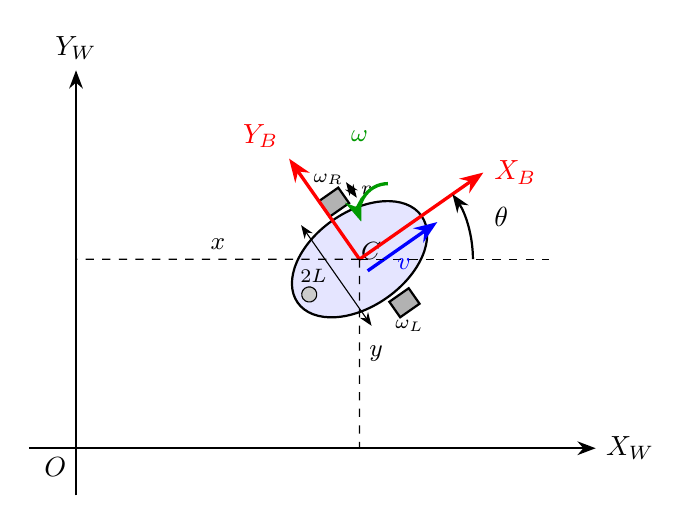
\begin{tikzpicture}[scale=1.2, >=Stealth]
    \draw[->, thick] (-0.5,0) -- (5.5,0) node[right] {$X_W$};
    \draw[->, thick] (0,-0.5) -- (0,4.0) node[above] {$Y_W$};
    \node[below left] at (0,0) {$O$};
    \coordinate (C) at (3, 2);
    \def\thetaR{35}
    \begin{scope}[shift={(C)}, rotate=\thetaR]
        \draw[fill=blue!10, thick] (0,0) ellipse (0.8 and 0.5);
        \node at (0.15,0) {\small $C$};
        \draw[fill=gray!60, thick] (0, 0.55) rectangle (0.25, 0.75);
        \node[above, font=\scriptsize] at (0.12, 0.75) {$\omega_R$};
        \draw[fill=gray!60, thick] (0, -0.75) rectangle (0.25, -0.55);
        \node[below, font=\scriptsize] at (0.12, -0.75) {$\omega_L$};
        \draw[fill=gray!40] (-0.65, 0) circle (0.08);
        \draw[->, red, very thick] (0,0) -- (1.6,0) node[right] {$X_B$};
        \draw[->, red, very thick] (0,0) -- (0,1.3) node[above left] {$Y_B$};
        \draw[->, blue, very thick] (0,-0.15) -- (0.9,-0.15);
        \node[blue, font=\small, below] at (0.45, -0.18) {$v$};
        \draw[<->, thin] (-0.3, -0.65) -- (-0.3, 0.65);
        \node[left, font=\scriptsize] at (-0.3, 0) {$2L$};
        \draw[<->, thin] (0.35, 0.55) -- (0.35, 0.75);
        \node[right, font=\scriptsize] at (0.35, 0.65) {$r$};
    \end{scope}
    \draw[dashed, thin] (C) -- ++(2.0, 0);
    \draw[->, thick] ($(C)+(1.2,0)$) arc[start angle=0, end angle=\thetaR, radius=1.2];
    \node at ($(C)+(1.5, 0.45)$) {$\theta$};
    \draw[->, green!60!black, very thick] ($(C)+(0.3,0.8)$) arc[start angle=90, end angle=200, radius=0.3];
    \node[green!60!black, font=\small] at ($(C)+(0.0,1.3)$) {$\omega$};
    \draw[dashed, thin] (C) -- (3, 0) node[midway, right, font=\small] {$y$};
    \draw[dashed, thin] (C) -- (0, 2) node[midway, above, font=\small] {$x$};
\end{tikzpicture}
\caption{Mô hình robot di động vi sai: hệ tọa độ quán tính $\{O, X_W, Y_W\}$, hệ tọa độ thân robot $\{C, X_B, Y_B\}$ (đỏ), vận tốc dài $v$ (xanh), vận tốc góc $\omega$ (xanh lá)}
\label{fig:wmr_schematic}
\end{figure}

\subsection*{2.2\quad Mô hình động lực học (Dynamic model)}
\addcontentsline{toc}{subsection}{2.2\quad Mô hình động lực học}

Mô hình động học (\ref{eq:kinematics}) giả thiết robot có thể đạt ngay lập tức bất kỳ vận tốc $(v, \omega)$ nào, bỏ qua quán tính và ma sát. Trong thực tế, để thay đổi vận tốc cần có lực (mô-men) từ động cơ, và ma sát cản trở chuyển động. Mô hình động lực học (Fierro \& Lewis \cite{Fierro1997}) mô tả mối quan hệ giữa mô-men đầu vào và gia tốc:
\begin{equation}\label{eq:dynamics}
    M\,\dot{\eta} = B\,\tau - F(\eta)
\end{equation}

Các ma trận và vector trong (\ref{eq:dynamics}) có ý nghĩa vật lý rõ ràng:

\textbf{Ma trận quán tính} $M = \diag(m, I)$: mô tả sức ỳ của robot. Thành phần $m$ (kg) là khối lượng tổng, quyết định lực cần thiết để thay đổi vận tốc dài. Thành phần $I$ (kg$\cdot$m$^2$) là mô-men quán tính quay quanh trục thẳng đứng, quyết định mô-men cần thiết để thay đổi vận tốc góc. $M$ là ma trận chéo vì giả thiết robot đối xứng qua trục dọc.

\textbf{Ma trận chuyển đổi mô-men} $B$:
\begin{equation}\label{eq:B_matrix}
    B = \begin{bmatrix} r/2 & r/2 \\ r/(2L) & -r/(2L) \end{bmatrix}
\end{equation}
chuyển đổi từ mô-men hai bánh $\tau = [\tau_R, \tau_L]^\T$ (N$\cdot$m) sang lực/mô-men tác dụng tại tâm robot. Hàng thứ nhất: lực đẩy dọc $F = (r/2)(\tau_R + \tau_L)$ (hai bánh cùng chiều tạo lực tiến). Hàng thứ hai: mô-men quay $N = (r/2L)(\tau_R - \tau_L)$ (hai bánh ngược chiều tạo quay).

\textbf{Vector ma sát} $F(\eta)$ mô hình hóa tổn thất ma sát:
\begin{equation}\label{eq:friction}
    F(\eta) = \begin{bmatrix} f_v \cdot v + f_c \cdot \tanh(v/\varepsilon) \\ f_\omega \cdot \omega + f_{c\omega} \cdot \tanh(\omega/\varepsilon) \end{bmatrix}
\end{equation}
bao gồm hai thành phần: (i) ma sát nhớt (viscous friction) $f_v \cdot v$ tỉ lệ thuận với vận tốc, mô hình hóa lực cản của dầu bôi trơn, ổ bi, và không khí; (ii) ma sát Coulomb $f_c \cdot \tanh(v/\varepsilon)$ xấp xỉ ma sát khô (gần hằng số khi có chuyển động), dùng $\tanh$ thay $\sign$ để tránh gián đoạn tại $v=0$ ($\varepsilon$ nhỏ, thường $\varepsilon = 0.01$).

\textbf{Tham số Pioneer 3-DX} (robot nghiên cứu phổ biến): $m = 10$\,kg, $I = 0.5$\,kg$\cdot$m$^2$, $r = 0.05$\,m, $L = 0.15$\,m, $\tau_\text{max} = 20$\,N$\cdot$m, $f_v = 0.5$, $f_c = 0.2$, $f_\omega = 0.3$, $f_{c\omega} = 0.1$.

\begin{table}[H]
\centering
\caption{Tham số robot Pioneer 3-DX sử dụng trong mô phỏng}
\label{tab:robot_params}
\begin{tabular}{llll}
\toprule
\textbf{Tham số} & \textbf{Ký hiệu} & \textbf{Giá trị} & \textbf{Đơn vị} \\
\midrule
Khối lượng & $m$ & 10 & kg \\
Mô-men quán tính & $I$ & 0.5 & kg$\cdot$m$^2$ \\
Bán kính bánh xe & $r$ & 0.05 & m \\
Nửa khoảng cách trục & $L$ & 0.15 & m \\
Mô-men tối đa & $\tau_\text{max}$ & 20 & N$\cdot$m \\
Ma sát nhớt (dài) & $f_v$ & 0.5 & N$\cdot$s/m \\
Ma sát Coulomb (dài) & $f_c$ & 0.2 & N \\
Ma sát nhớt (góc) & $f_\omega$ & 0.3 & N$\cdot$m$\cdot$s/rad \\
Ma sát Coulomb (góc) & $f_{c\omega}$ & 0.1 & N$\cdot$m \\
\bottomrule
\end{tabular}
\end{table}

Các tham số trên được lấy từ Pioneer 3-DX, một nền tảng robot di động phổ biến trong nghiên cứu, được sản xuất bởi Adept MobileRobots. Robot này có kích thước nhỏ gọn ($L \times W \times H = 455 \times 381 \times 237$\,mm), phù hợp cho thí nghiệm trong phòng lab. Tuy nhiên, trong thực tế, các tham số $m$ và $I$ thay đổi đáng kể khi robot mang tải -- đây chính là nguồn bất định khảo sát trong Phần B (Chương 5).

\subsection*{2.3\quad Mô hình ghép 5 trạng thái}
\addcontentsline{toc}{subsection}{2.3\quad Mô hình ghép 5 trạng thái}

Ghép mô hình động học (\ref{eq:kinematics}) và động lực học (\ref{eq:dynamics}), ta được mô hình đầy đủ 5 trạng thái $[x, y, \theta, v, \omega]^\T$:
\begin{equation}\label{eq:full_model}
    \frac{d}{dt}\begin{bmatrix} x \\ y \\ \theta \\ v \\ \omega \end{bmatrix}
    = \begin{bmatrix} v\cos\theta \\ v\sin\theta \\ \omega \\ \hdashline M^{-1}(B\tau - F(\eta)) \end{bmatrix}
\end{equation}

Mô hình (\ref{eq:full_model}) phản ánh đầy đủ vật lý robot: ba trạng thái đầu $(x, y, \theta)$ mô tả hình học (vị trí và hướng), hai trạng thái sau $(v, \omega)$ mô tả động lực (vận tốc). Đầu vào thực sự là mô-men $\tau = [\tau_R, \tau_L]^\T$ chứ không phải vận tốc $(v, \omega)$ như mô hình kinematic giả định. Sự phân biệt này rất quan trọng: trên mô hình kinematic, vận tốc thay đổi tức thời; trên mô hình đầy đủ, vận tốc thay đổi theo quán tính -- cần thời gian và năng lượng.

\subsection*{2.4\quad Sai số bám trong hệ tọa độ thân robot}
\addcontentsline{toc}{subsection}{2.4\quad Sai số bám trong hệ tọa độ thân robot}

Cho quỹ đạo tham chiếu $q_r(t) = [x_r, y_r, \theta_r]^\T$ với vận tốc $(v_r, \omega_r)$ thỏa mãn (\ref{eq:kinematics}). Sai số bám được biểu diễn trong hệ tọa độ thân robot (body frame) theo Kanayama et al. \cite{Kanayama1990}:
\begin{equation}\label{eq:error_def}
    z = \begin{bmatrix} z_x \\ z_y \\ z_\theta \end{bmatrix}
    = R(\theta) \begin{bmatrix} x_r - x \\ y_r - y \\ \theta_r - \theta \end{bmatrix}, \quad
    R(\theta) = \begin{bmatrix} \cos\theta & \sin\theta & 0 \\ -\sin\theta & \cos\theta & 0 \\ 0 & 0 & 1 \end{bmatrix}
\end{equation}

Ma trận $R(\theta)$ là phép quay chuyển từ world frame sang body frame. Ý nghĩa vật lý của các thành phần sai số:

\begin{itemize}
    \item $z_x$ -- \textbf{sai số dọc (along-track error):} khoảng cách từ robot đến điểm tham chiếu chiếu theo hướng tiến của robot. $z_x > 0$ nghĩa là điểm tham chiếu ở phía trước, robot cần tăng tốc để bắt kịp.

    \item $z_y$ -- \textbf{sai số ngang (cross-track error):} khoảng cách lệch ngang so với quỹ đạo tham chiếu. $z_y > 0$ nghĩa là quỹ đạo ở bên trái, robot cần lệch trái.

    \item $z_\theta$ -- \textbf{sai số góc (heading error):} chênh lệch góc hướng. $z_\theta > 0$ nghĩa là robot cần quay phải (ngược chiều kim đồng hồ) để hướng đúng.
\end{itemize}

\textbf{Tại sao dùng body frame thay vì world frame?} Biểu diễn sai số trong body frame có hai ưu điểm quan trọng: (i) các thành phần sai số có ý nghĩa vật lý trực quan gắn với hành vi robot (trước/sau, trái/phải); (ii) quan trọng hơn, phương trình động lực học sai số trong body frame có dạng affine $\dot{z} = f(z, u_r) + g(z) u_o$ thuận lợi cho thiết kế ADP, trong khi dạng trong world frame phức tạp hơn do phụ thuộc tường minh vào $\theta$.

Hình~\ref{fig:error_body_frame} minh họa các thành phần sai số trong body frame.

\begin{figure}[H]
\centering
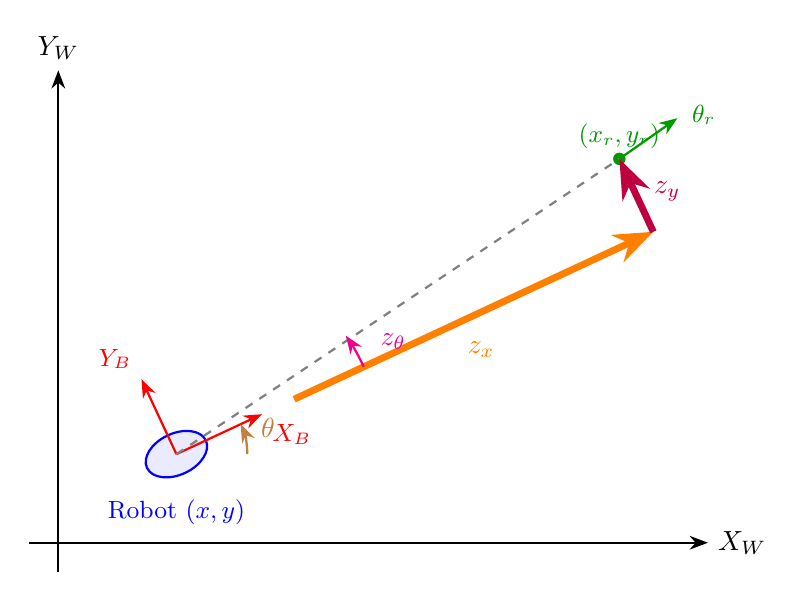
\begin{tikzpicture}[scale=0.75, >=Stealth]
    % World frame
    \draw[->, thick] (-0.5,0) -- (11,0) node[right] {$X_W$};
    \draw[->, thick] (0,-0.5) -- (0,8) node[above] {$Y_W$};

    % Actual position
    \coordinate (A) at (2, 1.5);
    \def\thetaA{25}

    % Robot body
    \begin{scope}[shift={(A)}, rotate=\thetaA]
        \draw[blue, thick, fill=blue!8] (0,0) ellipse (0.55 and 0.35);
        % Body frame axes (short, clear labels away from error arrows)
        \draw[->, red, thick] (0,0) -- (1.6,0) node[below right, font=\small] {$X_B$};
        \draw[->, red, thick] (0,0) -- (0,1.4) node[above left, font=\small] {$Y_B$};
    \end{scope}
    \node[below, blue, font=\small] at ($(A)+(0,-0.6)$) {Robot $(x, y)$};

    % Theta arc (close to robot, small radius to avoid overlap with error arrows)
    \draw[->, thick, brown] ($(A)+(1.2,0)$) arc[start angle=0, end angle=\thetaA, radius=1.2];
    \node[brown, font=\bfseries] at ($(A)+(1.55,0.45)$) {$\theta$};

    % Reference position (far away)
    \coordinate (R) at (9.5, 6.5);
    \fill[green!60!black] (R) circle (3pt);
    \node[above, green!60!black, font=\small] at (R) {$(x_r, y_r)$};
    \draw[->, green!60!black, thick] (R) -- ++(35:1.2);
    \node[green!60!black, font=\small, right] at ($(R)+(35:1.3)$) {$\theta_r$};

    % Error vector (dashed world frame)
    \draw[dashed, gray, thick] (A) -- (R);

    % Error components in body frame
    \begin{scope}[shift={(A)}, rotate=\thetaA]
        \pgfmathsetmacro{\exW}{9.5-2}
        \pgfmathsetmacro{\eyW}{6.5-1.5}
        \pgfmathsetmacro{\cosT}{cos(\thetaA)}
        \pgfmathsetmacro{\sinT}{sin(\thetaA)}
        \pgfmathsetmacro{\zx}{\exW*\cosT + \eyW*\sinT}
        \pgfmathsetmacro{\zy}{-\exW*\sinT + \eyW*\cosT}

        % z_x (along X_B, start well past X_B label)
        \draw[->, orange, line width=2.5pt] (2.2,0) -- (\zx, 0);
        \node[orange, font=\bfseries, below] at ({(\zx+2.2)/2}, -0.3) {$z_x$};

        % z_y (perpendicular, from tip of z_x)
        \draw[->, purple, line width=2.5pt] (\zx, 0) -- (\zx, \zy);
        \node[purple, font=\bfseries, right] at (\zx+0.15, \zy/2) {$z_y$};
    \end{scope}

    % z_theta arc between theta_r and theta directions
    \draw[->, magenta, thick] ($(A)+(25:3.5)$) arc[start angle=25, end angle=35, radius=3.5];
    \node[magenta, font=\bfseries, right] at ($(A)+(30:3.8)$) {$z_\theta$};

\end{tikzpicture}
\caption{Sai số bám trong hệ tọa độ thân robot: $z_x$ (cam) là sai số dọc theo $X_B$, $z_y$ (tím) là sai số ngang theo $Y_B$, $z_\theta = \theta_r - \theta$ là sai số góc hướng}
\label{fig:error_body_frame}
\end{figure}

\subsection*{2.5\quad Động lực học sai số}
\addcontentsline{toc}{subsection}{2.5\quad Động lực học sai số}

Đặt luật điều khiển tổng quát dạng feedforward + feedback:
\begin{equation}\label{eq:control_split}
    u = u_f + u_o = \begin{bmatrix} v_r\cos z_\theta \\ \omega_r \end{bmatrix} + \begin{bmatrix} u_{o1} \\ u_{o2} \end{bmatrix}
\end{equation}

Phần feedforward $u_f = [v_r\cos z_\theta,\ \omega_r]^\T$ bù đường đi danh nghĩa, phần feedback $u_o = [u_{o1},\ u_{o2}]^\T$ hiệu chỉnh sai số. Lấy đạo hàm (\ref{eq:error_def}) theo thời gian và thay thế (\ref{eq:kinematics}), ta được động lực học sai số:
\begin{equation}\label{eq:error_dynamics}
    \boxed{\dot{z} = f(z, u_r) + g(z)\, u_o}
\end{equation}
với:
\begin{equation}\label{eq:f_and_g}
    f(z, u_r) = \begin{bmatrix} z_y\omega_r \\ -z_x\omega_r + v_r\sin z_\theta \\ 0 \end{bmatrix}, \quad
    g(z) = \begin{bmatrix} -1 & z_y \\ 0 & -z_x \\ 0 & -1 \end{bmatrix}
\end{equation}

\textbf{Chứng minh chi tiết.} Lấy đạo hàm thành phần đầu tiên $z_x$:
\begin{align}
    \dot{z}_x &= \frac{d}{dt}\big[\cos\theta(x_r - x) + \sin\theta(y_r - y)\big] \nonumber \\
    &= -\omega\sin\theta(x_r - x) + \cos\theta(\dot{x}_r - \dot{x})
    + \omega\cos\theta(y_r - y) + \sin\theta(\dot{y}_r - \dot{y}) \nonumber \\
    &= \omega z_y + v_r\cos z_\theta - v \nonumber \\
    &= z_y\omega_r + z_y u_{o2} - u_{o1} \label{eq:zx_deriv}
\end{align}
trong đó đã sử dụng $\omega = \omega_r + u_{o2}$ và $v = v_r\cos z_\theta + u_{o1}$.

Tương tự cho $z_y$:
\begin{align}
    \dot{z}_y &= -z_x\omega_r - z_x u_{o2} + v_r\sin z_\theta \label{eq:zy_deriv}
\end{align}

Và cho $z_\theta$:
\begin{align}
    \dot{z}_\theta &= \omega_r - \omega = -u_{o2} \label{eq:ztheta_deriv}
\end{align}

Tổng hợp (\ref{eq:zx_deriv})--(\ref{eq:ztheta_deriv}) cho dạng (\ref{eq:error_dynamics})--(\ref{eq:f_and_g}).

\textbf{Phân tích cấu trúc hệ sai số:}

\begin{itemize}
    \item $u_{o1}$ tác động \textit{trực tiếp} lên $z_x$ (hệ số $-1$ trong $g$), phản ánh việc điều chỉnh vận tốc dài ảnh hưởng ngay lập tức đến sai số dọc.

    \item $u_{o2}$ tác động trực tiếp lên cả $z_x$ (qua $z_y u_{o2}$, ghép nối nonholonomic), $z_y$ (qua $-z_x u_{o2}$), và $z_\theta$ (trực tiếp, hệ số $-1$). Điều này cho thấy vận tốc góc là kênh điều khiển ``mạnh hơn'', ảnh hưởng đồng thời ba thành phần sai số.

    \item \textbf{Hiện tượng cascade nonholonomic:} Sai số ngang $z_y$ không có kênh điều khiển trực tiếp riêng. Nó hội tụ \textit{gián tiếp} thông qua thành phần $v_r\sin z_\theta$ -- khi $z_\theta$ khác không, thành phần $v_r\sin z_\theta$ ``kéo'' $z_y$ về không. Đây là đặc trưng của hệ nonholonomic: không thể di chuyển ngang trực tiếp mà phải quay rồi tiến.
\end{itemize}

Hệ (\ref{eq:error_dynamics}) có dạng phi tuyến affine (affine in control), đây chính xác là dạng cần thiết để áp dụng Approximate Dynamic Programming (ADP).

\subsection*{2.6\quad Quỹ đạo tham chiếu}
\addcontentsline{toc}{subsection}{2.6\quad Quỹ đạo tham chiếu}

Luận văn sử dụng ba loại quỹ đạo tham chiếu với đặc tính khác nhau để đánh giá toàn diện các bộ điều khiển:

\textbf{Đường tròn:} Tâm $(0, 0)$, bán kính $R_c = 2$\,m, vận tốc dài $v_r = 0.3$\,m/s:
\begin{equation}\label{eq:ref_circle}
    x_r = R_c\cos(\omega_c t), \quad y_r = R_c\sin(\omega_c t), \quad \omega_c = v_r/R_c = 0.15\,\text{rad/s}
\end{equation}
Đường tròn có độ cong hằng số $\kappa = 1/R_c$, thích hợp để đánh giá hiệu năng bám ở chế độ xác lập.

\textbf{Đường thẳng:} Vận tốc dài $v_r = 0.3$\,m/s, $\omega_r = 0$:
\begin{equation}\label{eq:ref_line}
    x_r = v_r t, \quad y_r = 0, \quad \theta_r = 0
\end{equation}
Đường thẳng là trường hợp đơn giản nhất ($\omega_r = 0$), tuy nhiên cũng kiểm tra khả năng hội tụ transient vì sai số ban đầu vẫn khác không.

\textbf{Hình số 8 (lemniscate):} Quỹ đạo phức tạp với độ cong biến thiên liên tục, bao gồm cả điểm đổi chiều:
\begin{equation}\label{eq:ref_fig8}
    x_r = 2\sin(\omega_8 t), \quad y_r = \sin(2\omega_8 t), \quad \omega_8 = 0.1\,\text{rad/s}
\end{equation}
Hình số 8 là bài kiểm tra khắt khe nhất vì: (i) độ cong thay đổi liên tục, đòi hỏi bộ điều khiển thích nghi nhanh; (ii) tại điểm giao ($t = k\pi/\omega_8$), $\omega_r$ đổi dấu đột ngột; (iii) vận tốc tham chiếu biến thiên theo thời gian.

\begin{figure}[H]
\centering
\begin{tikzpicture}
\begin{axis}[
    width=9cm, height=7cm,
    xlabel={$x$ (m)}, ylabel={$y$ (m)},
    xmin=-3, xmax=5, ymin=-2.8, ymax=2.8,
    legend style={at={(1.02,0.5)}, anchor=west, font=\small},
    grid=major, grid style={gray!20},
    axis equal image,
    thick
]
% Circle
\addplot[blue, very thick, domain=0:360, samples=200] ({2*cos(x)}, {2*sin(x)});
\addlegendentry{Đường tròn ($R_c=2$\,m)}

% Line
\addplot[red, very thick, dashed, domain=0:5] (x, 0);
\addlegendentry{Đường thẳng ($v_r=0.3$\,m/s)}

% Figure-8
\addplot[green!60!black, very thick, dashdotted, domain=0:360, samples=300] ({2*sin(x)}, {sin(2*x)});
\addlegendentry{Hình số 8 (lemniscate)}

% Start points
\addplot[only marks, mark=*, mark size=3pt, blue] coordinates {(2, 0)};
\addplot[only marks, mark=*, mark size=3pt, red] coordinates {(0, 0)};
\addplot[only marks, mark=*, mark size=3pt, green!60!black] coordinates {(0, 0)};

\end{axis}
\end{tikzpicture}
\caption{Ba loại quỹ đạo tham chiếu sử dụng trong mô phỏng: đường tròn (độ cong hằng số), đường thẳng (đơn giản nhất), và hình số 8 (độ cong biến thiên, có điểm đổi chiều)}
\label{fig:ref_trajectories}
\end{figure}


% ================================================================
% CHƯƠNG 3: CƠ SỞ LÝ THUYẾT ĐIỀU KHIỂN TỐI ƯU VÀ ADP
% ================================================================
\newpage
\setchapter{3}
\section*{CHƯƠNG 3: CƠ SỞ LÝ THUYẾT ĐIỀU KHIỂN TỐI ƯU VÀ ADP}
\addcontentsline{toc}{section}{CHƯƠNG 3: CƠ SỞ LÝ THUYẾT ĐIỀU KHIỂN TỐI ƯU VÀ ADP}

\subsection*{3.1\quad Bài toán điều khiển tối ưu và phương trình HJB}
\addcontentsline{toc}{subsection}{3.1\quad Bài toán điều khiển tối ưu và phương trình HJB}

Xét hệ phi tuyến affine dạng tổng quát $\dot{z} = f(z) + g(z) u_o$, $z \in \R^n$, $u_o \in \R^m$. Bài toán điều khiển tối ưu đặt ra: tìm chính sách điều khiển phản hồi $u_o^*(z)$ cực tiểu hóa hàm chi phí vô hạn:
\begin{equation}\label{eq:cost}
    J(z_0, u_o) = \int_0^\infty \big( z^\T Q\, z + u_o^\T R\, u_o \big)\, dt
\end{equation}
trong đó $z_0$ là trạng thái ban đầu, $Q = Q^\T \geq 0$ là ma trận trọng số trạng thái (bán xác định dương), và $R = R^\T > 0$ là ma trận trọng số điều khiển (xác định dương).

\textbf{Nguyên lý tối ưu Bellman:} Định nghĩa hàm giá trị tối ưu $V^*(z) = \min_{u_o} J(z, u_o)$. Theo nguyên lý tối ưu Bellman (Bellman's principle of optimality), nếu $u_o^*$ là chính sách tối ưu, thì mọi ``đoạn con'' của nó cũng phải tối ưu. Điều kiện cần và đủ cho $V^*(z)$ được biểu diễn bởi phương trình Hamilton-Jacobi-Bellman (HJB):
\begin{equation}\label{eq:hjb}
    0 = \min_{u_o} \Big\{ z^\T Q z + u_o^\T R u_o + (\nabla V^*)^\T (f + g\, u_o) \Big\}
\end{equation}

Lấy đạo hàm biểu thức trong dấu $\min$ theo $u_o$ và cho bằng không, ta được điều khiển tối ưu:
\begin{equation}\label{eq:optimal_u}
    u_o^*(z) = -\frac{1}{2} R^{-1}\, g(z)^\T\, \nabla V^*(z)
\end{equation}

Thay (\ref{eq:optimal_u}) ngược vào (\ref{eq:hjb}), ta được dạng rút gọn:
\begin{equation}\label{eq:hjb_reduced}
    0 = z^\T Q z + (\nabla V^*)^\T f - \frac{1}{4} (\nabla V^*)^\T g R^{-1} g^\T \nabla V^*
\end{equation}

Phương trình (\ref{eq:hjb_reduced}) là một phương trình đạo hàm riêng (PDE) phi tuyến bậc nhất đối với $V^*(z)$. Trong trường hợp hệ tuyến tính $\dot{z} = Az + Bu_o$, phương trình HJB trở thành phương trình đại số Riccati (Algebraic Riccati Equation -- ARE), có nghiệm giải tích. Tuy nhiên, đối với hệ phi tuyến như WMR, phương trình HJB \textbf{không giải được bằng giải tích} trừ vài trường hợp đặc biệt. Đây chính là động lực cho Quy hoạch động xấp xỉ (ADP).

\textbf{So sánh với LQR:} Đối với hệ tuyến tính $\dot{z} = Az + Bu$, hàm chi phí bậc hai $J = \int(z^\T Qz + u^\T Ru)dt$, nghiệm tối ưu là $u^* = -Kz$ với $K = R^{-1}B^\T P$ và $P$ là nghiệm ARE $A^\T P + PA - PBR^{-1}B^\T P + Q = 0$. Đây là bài toán giải được hoàn toàn. ADP có thể coi là ``LQR mở rộng cho hệ phi tuyến'' -- xấp xỉ hàm $V^*$ (tương ứng $z^\T Pz$ trong LQR) bằng mạng nơ-ron thay vì giải ARE.

\textbf{Hai kiến trúc ADP chính:} Trong nghiên cứu ADP, có hai kiến trúc phổ biến:

\begin{itemize}
    \item \textbf{Actor-Critic (AC):} Sử dụng hai mạng nơ-ron riêng biệt -- mạng Critic ước lượng $V(z)$, mạng Actor ước lượng $u_o(z)$. Hai mạng cập nhật đồng thời: Critic giảm sai số Bellman, Actor giảm sai lệch chính sách. Ưu điểm: linh hoạt, actor có thể xấp xỉ chính sách phức tạp không suy trực tiếp từ $\nabla V$. Nhược điểm: cần đồng bộ hai mạng (nếu actor ``chạy trước'' critic hoặc ngược lại, cả hai có thể phân kỳ), nhiều siêu tham số ($\alpha_c, \alpha_{a1}, \alpha_{a2}, \kappa_c$), và yêu cầu PE.

    \item \textbf{Critic-only:} Chỉ sử dụng một mạng Critic, chính sách $u_o$ suy trực tiếp từ $\nabla V$ qua (\ref{eq:optimal_u}). Ưu điểm: ít siêu tham số hơn, không cần đồng bộ, có thể kết hợp Concurrent Learning để loại bỏ PE. Nhược điểm: chính sách phụ thuộc hoàn toàn vào chất lượng xấp xỉ $V$ -- nếu basis functions $\phi$ không phù hợp, cả $V$ và $u_o$ đều kém.
\end{itemize}

Luận văn sử dụng cả hai kiến trúc để so sánh: Actor-Critic (phương pháp 2) và Critic-only (phương pháp 4 CL, phương pháp 5 ADP-FT).

\begin{figure}[H]
\centering
\resizebox{0.95\textwidth}{!}{%
\begin{tikzpicture}[
    block/.style={draw, thick, minimum width=2.2cm, minimum height=0.9cm, align=center, rounded corners=3pt, font=\small},
    arrow/.style={->, >=Stealth, thick},
    node distance=1.2cm
]
    % Plant
    \node[block, fill=blue!10] (plant) {Hệ thống\\$\dot{z}=f+g\,u_o$};

    % Critic
    \node[block, fill=orange!15, right=2.2cm of plant] (critic) {Mạng Critic\\$\hat{V}=W^\T\phi(z)$};

    % Policy
    \node[block, fill=green!15, below=1.2cm of critic] (policy) {Chính sách\\$u_o=-\frac{1}{2}R^{-1}g^\T\nabla\phi^\T W$};

    % Weight update
    \node[block, fill=red!10, above=1.2cm of critic] (update) {Cập nhật $W$\\$\dot{W}=-\alpha\bar{\sigma}\delta-\kappa W$};

    % Bellman error
    \node[block, fill=yellow!15, right=1.8cm of critic] (bellman) {Sai số Bellman\\$\delta=W^\T\sigma+z^\T Qz+u_o^\T Ru_o$};

    % Arrows
    \draw[arrow] (plant) -- node[above, font=\scriptsize] {$z(t)$} (critic);
    \draw[arrow] (critic) -- node[right, font=\scriptsize] {$\nabla V$} (policy);
    \draw[arrow] (policy.west) -| node[below left, font=\scriptsize] {$u_o$} (plant.south);
    \draw[arrow] (critic) -- node[above, font=\scriptsize] {$W, \sigma$} (bellman);
    \draw[arrow] (bellman) |- node[above right, font=\scriptsize] {$\delta$} (update);
    \draw[arrow] (update) -- node[left, font=\scriptsize] {$W$} (critic);

\end{tikzpicture}%
}
\caption{Cấu trúc Critic-only ADP: mạng Critic xấp xỉ hàm giá trị, chính sách suy trực tiếp từ gradient $\nabla V$, trọng số cập nhật theo sai số Bellman}
\label{fig:adp_structure}
\end{figure}

\subsection*{3.2\quad Quy hoạch động xấp xỉ (Approximate Dynamic Programming)}
\addcontentsline{toc}{subsection}{3.2\quad Quy hoạch động xấp xỉ (ADP)}

Ý tưởng cốt lõi của ADP là xấp xỉ hàm giá trị tối ưu $V^*(z)$ bằng tổ hợp tuyến tính của các hàm cơ sở (basis functions):
\begin{equation}\label{eq:approx_V}
    V^*(z) \approx W^{*\T} \phi(z) + \varepsilon_\phi(z)
\end{equation}
trong đó $W^* \in \R^l$ là vector trọng số tối ưu (chưa biết), $\phi(z) \in \R^l$ là vector các hàm cơ sở đã chọn trước, và $\varepsilon_\phi$ là sai số xấp xỉ (nhỏ nếu $\phi$ được chọn phù hợp).

\textbf{Lựa chọn hàm cơ sở:} Đối với hệ sai số WMR với $z \in \R^3$, ta chọn $l = 6$ hàm cơ sở bậc hai:
\begin{equation}\label{eq:basis}
    \phi(z) = [z_x^2,\; z_y^2,\; z_\theta^2,\; z_x z_y,\; z_y z_\theta,\; z_x z_\theta]^\T \in \R^6
\end{equation}

Lựa chọn này có cơ sở lý thuyết: nếu hệ tuyến tính, $V^* = z^\T Pz$ là bậc hai, và $\phi$ bậc hai đủ để biểu diễn chính xác. Đối với hệ phi tuyến yếu (weakly nonlinear), $\phi$ bậc hai vẫn cho xấp xỉ tốt. Ngoài ra, $\phi(0) = 0$ đảm bảo $V^*(0) = 0$ (chi phí bằng không tại gốc).

\textbf{Ma trận Jacobian} $\nabla\phi(z) = \partial\phi/\partial z \in \R^{6 \times 3}$:
\begin{equation}\label{eq:nabla_phi}
    \nabla\phi = \begin{bmatrix}
        2z_x & 0 & 0 \\ 0 & 2z_y & 0 \\ 0 & 0 & 2z_\theta \\
        z_y & z_x & 0 \\ 0 & z_\theta & z_y \\ z_\theta & 0 & z_x
    \end{bmatrix}
\end{equation}

Jacobian $\nabla\phi$ đóng vai trò trung tâm: $\nabla V^* \approx \nabla\phi^\T W^*$, cho phép tính luật điều khiển xấp xỉ:
\begin{equation}\label{eq:adp_control}
    \hat{u}_o = -\frac{1}{2} R^{-1} g(z)^\T \nabla\phi(z)^\T W
\end{equation}
trong đó $W$ là ước lượng hiện tại của $W^*$, được cập nhật trực tuyến.

\subsection*{3.3\quad Sai số Bellman (Bellman error)}
\addcontentsline{toc}{subsection}{3.3\quad Sai số Bellman}

Thay xấp xỉ $V \approx W^\T\phi$ vào phương trình HJB (\ref{eq:hjb_reduced}), sai số (residual) được gọi là sai số Bellman:
\begin{equation}\label{eq:bellman_error}
    \delta = W^\T \sigma + z^\T Q z + \hat{u}_o^\T R \hat{u}_o
\end{equation}
trong đó $\sigma = \nabla\phi(f + g\hat{u}_o)$ là vector ``đặc trưng thời gian'' (temporal feature), phản ánh tốc độ thay đổi xấp xỉ $V$ dọc theo quỹ đạo hệ.

Khi $W = W^*$ (trọng số tối ưu), sai số Bellman $\delta = 0$ -- nghĩa là phương trình HJB được thỏa mãn chính xác (bỏ qua sai số xấp xỉ $\varepsilon_\phi$). Do đó, mục tiêu của các thuật toán ADP là cập nhật $W$ sao cho $\delta \to 0$, tương đương $W \to W^*$.

Ký hiệu chuẩn hóa thường dùng:
\begin{equation}\label{eq:sigma_bar}
    \bar{\sigma} = \frac{\sigma}{(1 + \sigma^\T \sigma)^2}
\end{equation}
để tránh phân kỳ số khi $\|\sigma\|$ lớn. Hệ số $(1 + \sigma^\T\sigma)^2$ ở mẫu đảm bảo $\|\bar{\sigma}\|$ luôn bị chặn.

\subsection*{3.4\quad Ổn định cố định thời gian (Fixed-time stability)}
\addcontentsline{toc}{subsection}{3.4\quad Ổn định cố định thời gian}

\textbf{Định nghĩa (Polyakov \cite{Polyakov2012}):} Gốc $x = 0$ của hệ $\dot{x} = h(x)$ được gọi là ổn định cố định thời gian (fixed-time stable) nếu tồn tại hằng số $T_f > 0$ \textbf{không phụ thuộc vào điều kiện ban đầu} $x(0)$ sao cho $\|x(t)\| = 0$ với mọi $t \geq T_f$.

So sánh ba loại ổn định:

\begin{itemize}
    \item \textbf{Ổn định tiệm cận (asymptotic stability):} $\|x(t)\| \to 0$ khi $t \to \infty$. Sai số giảm dần nhưng không bao giờ chính xác bằng không trong thời gian hữu hạn. Ví dụ: $\dot{x} = -kx$ cho nghiệm $x(t) = x_0 e^{-kt}$.

    \item \textbf{Ổn định thời gian hữu hạn (finite-time stability):} $\|x(t)\| = 0$ với mọi $t \geq T_f(x_0)$, nhưng $T_f$ \textit{phụ thuộc vào điều kiện đầu} -- sai số ban đầu càng lớn, thời gian hội tụ càng lâu, và $T_f$ có thể tùy ý lớn. Ví dụ: $\dot{x} = -\alpha|x|^p \sign(x)$, $0 < p < 1$, cho $T_f = |x_0|^{1-p}/[\alpha(1-p)]$.

    \item \textbf{Ổn định cố định thời gian (fixed-time stability):} $\|x(t)\| = 0$ với mọi $t \geq T_f$, và $T_f$ là hằng số \textit{độc lập với $x(0)$}. Đây là tính chất mạnh nhất, đảm bảo hiệu năng trong mọi tình huống.
\end{itemize}

\textbf{Lemma quan trọng:} Nếu tồn tại hàm Lyapunov $V(x) > 0$ ($V(0) = 0$) sao cho:
\begin{equation}\label{eq:ft_lyapunov}
    \dot{V} \leq -\alpha V^p - \beta V^q, \quad 0 < p < 1 < q, \quad \alpha, \beta > 0
\end{equation}
thì hệ ổn định cố định thời gian với cận trên:
\begin{equation}\label{eq:ft_bound}
    T_f \leq \frac{1}{\alpha(1-p)} + \frac{1}{\beta(q-1)}
\end{equation}

Ý nghĩa vật lý: thành phần $-\alpha V^p$ (lũy thừa phân số, $p < 1$) chi phối khi $V$ nhỏ (gần gốc), đảm bảo hội tụ nhanh trong ``vùng lân cận cuối cùng'' -- nơi mà ổn định tiệm cận trở nên chậm. Thành phần $-\beta V^q$ (lũy thừa bậc cao, $q > 1$) chi phối khi $V$ lớn (xa gốc), đảm bảo hội tụ nhanh từ điều kiện đầu lớn. Sự kết hợp hai thành phần tạo nên cận trên $T_f$ không phụ thuộc $V(0)$.

\begin{figure}[H]
\centering
\begin{tikzpicture}
\begin{axis}[
    width=11cm, height=6.5cm,
    xlabel={Thời gian $t$ (s)},
    ylabel={$\|x(t)\|$},
    xmin=0, xmax=6, ymin=-0.05, ymax=1.1,
    legend style={at={(0.98,0.98)}, anchor=north east, font=\small},
    grid=major, grid style={gray!30},
    thick
]
\addplot[blue, very thick, domain=0:6, samples=100] {exp(-0.5*x)};
\addlegendentry{Tiệm cận (Asymptotic)}
\addplot[red, very thick, dashed, domain=0:6, samples=100] {max(0, (1 - 0.35*x)^(2.5))};
\addlegendentry{Thời gian hữu hạn (Finite-time)}
\addplot[green!60!black, very thick, dashdotted, domain=0:6, samples=100] {max(0, (1 - 0.55*x)^(1.8))};
\addlegendentry{Cố định thời gian (Fixed-time)}
\draw[black, dashed, thin] (axis cs:1.82,-0.05) -- (axis cs:1.82,0.5);
\node[font=\small] at (axis cs:1.82,-0.12) {$T_f$};
\addplot[blue, thick, domain=0:6, samples=100, opacity=0.4] {0.5*exp(-0.5*x)};
\addplot[red, thick, dashed, domain=0:6, samples=100, opacity=0.4] {max(0, 0.5*(1 - 0.25*x)^(2.5))};
\addplot[green!60!black, thick, dashdotted, domain=0:6, samples=100, opacity=0.4] {max(0, 0.5*(1 - 0.8*x)^(1.8))};
\end{axis}
\end{tikzpicture}
\caption{So sánh ba loại ổn định. Đường đậm: $x_0 = 1$; đường mờ: $x_0 = 0.5$. Fixed-time hội tụ tại cùng $T_f$ bất kể $x_0$, trong khi finite-time phụ thuộc $x_0$, và asymptotic không bao giờ đạt 0.}
\label{fig:convergence_compare}
\end{figure}

\subsection*{3.5\quad Concurrent Learning (thay thế PE)}
\addcontentsline{toc}{subsection}{3.5\quad Concurrent Learning (thay thế PE)}

\textbf{Vấn đề Persistence of Excitation (PE):} Trong các phương pháp ADP truyền thống (Actor-Critic), để đảm bảo trọng số $W$ hội tụ về giá trị tối ưu $W^*$, cần điều kiện PE: tín hiệu đặc trưng $\sigma(t)$ phải ``đủ phong phú'' theo mọi hướng trong không gian $\R^l$. Chính thức:
\begin{equation}\label{eq:PE_condition}
    \exists \, T, \alpha_0 > 0: \quad \int_t^{t+T} \sigma(\tau)\sigma(\tau)^\T d\tau \geq \alpha_0 I, \quad \forall t \geq 0
\end{equation}

Điều kiện PE tạo ra mâu thuẫn cơ bản với bài toán bám quỹ đạo: khi bộ điều khiển hoạt động tốt ($z \to 0$), $\sigma \to 0$, và PE bị vi phạm. Để duy trì PE, cần thêm tín hiệu kích thích nhân tạo (probing signal), gây ra sai số bám bổ sung không mong muốn.

\textbf{Concurrent Learning (CL)} (Chowdhary \& Johnson \cite{Chowdhary2010}) giải quyết vấn đề này bằng cách lưu trữ dữ liệu lịch sử và sử dụng lại:

\begin{enumerate}
    \item \textbf{History stack:} Lưu bộ dữ liệu $\mathcal{H} = \{(\sigma_j, c_j)\}_{j=1}^{N_H}$ tại các thời điểm lấy mẫu trước đó, trong đó $c_j = z_j^\T Q z_j + \hat{u}_{o,j}^\T R \hat{u}_{o,j}$ là chi phí tức thời.

    \item \textbf{Luật cập nhật:} Kết hợp gradient trực tuyến (online) và gradient từ lịch sử (history):
    \begin{equation}\label{eq:cl_update}
        \dot{W} = -\alpha\bar{\sigma}\delta - \frac{\alpha_h}{N_H}\sum_{j=1}^{N_H} \bar{\sigma}_j \delta_j - \kappa W
    \end{equation}
    trong đó thành phần thứ hai tính sai số Bellman $\delta_j$ tại các điểm lịch sử bằng trọng số hiện tại $W$.

    \item \textbf{Điều kiện hội tụ:} Thay vì PE, CL chỉ cần điều kiện rank:
    \begin{equation}\label{eq:rank_condition}
        \rank\left(\sum_{j=1}^{N_H} \bar{\sigma}_j \bar{\sigma}_j^\T\right) = l
    \end{equation}
    nghĩa là tập dữ liệu lịch sử phải ``trải đều'' $l$ hướng trong không gian đặc trưng. Điều kiện này dễ thỏa mãn hơn PE rất nhiều: chỉ cần dữ liệu từ giai đoạn transient ban đầu (khi $z$ lớn và $\sigma$ phong phú), và được giữ vĩnh viễn trong history stack.
\end{enumerate}

Ưu điểm then chốt của CL: sau giai đoạn transient, dữ liệu lịch sử tiếp tục cung cấp thông tin gradient ngay cả khi $\sigma(t) \approx 0$ (bám tốt), cho phép trọng số tiếp tục hội tụ mà không cần tín hiệu kích thích.

\begin{figure}[H]
\centering
\begin{tikzpicture}[
    block/.style={draw, thick, minimum width=2.2cm, minimum height=0.9cm, align=center, rounded corners=2pt},
    arrow/.style={->, >=Stealth, thick},
    node distance=1.0cm
]
    % Online branch
    \node[block, fill=blue!10] (online) {Dữ liệu online\\$(\sigma(t), c(t))$};

    % History stack
    \node[block, fill=orange!15, below=1.2cm of online] (history) {History Stack\\$\{(\sigma_j, c_j)\}_{j=1}^{N_H}$};

    % Gradient online
    \node[block, fill=green!10, right=1.8cm of online] (grad_on) {Gradient online\\$-\alpha\bar\sigma\delta$};

    % Gradient history
    \node[block, fill=green!10, right=1.8cm of history] (grad_hist) {Gradient history\\$-\frac{\alpha_h}{N_H}\sum\bar\sigma_j\delta_j$};

    % Sum
    \node[draw, circle, thick, right=1.2cm of $(grad_on)!0.5!(grad_hist)$, minimum size=0.6cm] (sum) {$+$};

    % Weight update
    \node[block, fill=red!10, right=1.0cm of sum] (wdot) {$\dot{W}$};

    % Arrows
    \draw[arrow] (online) -- (grad_on);
    \draw[arrow] (history) -- (grad_hist);
    \draw[arrow] (grad_on) -| (sum);
    \draw[arrow] (grad_hist) -| (sum);
    \draw[arrow] (sum) -- (wdot);

    % Store arrow
    \draw[arrow, dashed] (online.south) -- node[left, font=\scriptsize] {lưu trữ} (history.north);

    % Labels
    \node[font=\scriptsize, gray, below=0.1cm of history] {Chỉ cần điều kiện rank, không cần PE};

\end{tikzpicture}
\caption{Concurrent Learning: kết hợp gradient online và gradient từ dữ liệu lịch sử, loại bỏ yêu cầu Persistence of Excitation}
\label{fig:cl_concept}
\end{figure}


% ================================================================
% CHƯƠNG 4: THIẾT KẾ HỆ THỐNG ĐIỀU KHIỂN
% ================================================================
\newpage
\setchapter{4}
\section*{CHƯƠNG 4: THIẾT KẾ HỆ THỐNG ĐIỀU KHIỂN}
\addcontentsline{toc}{section}{CHƯƠNG 4: THIẾT KẾ HỆ THỐNG ĐIỀU KHIỂN}

\subsection*{4.1\quad Kiến trúc hai vòng}
\addcontentsline{toc}{subsection}{4.1\quad Kiến trúc hai vòng}

Thiết kế điều khiển cho WMR trên mô hình đầy đủ 5 trạng thái đòi hỏi xử lý cả phần hình học (kinematic) lẫn phần động lực (dynamic). Luận văn sử dụng kiến trúc hai vòng (dual-loop), chia bài toán thành hai phần:

\textbf{Nguyên lý tách thang thời gian (separation of timescales):} Vòng trong được thiết kế nhanh hơn vòng ngoài (gains vòng trong $K_d = 20$ lớn hơn nhiều so với gains vòng ngoài). Nhờ vậy, từ góc nhìn vòng ngoài, vận tốc thực $(v, \omega)$ ``bám kịp'' vận tốc mong muốn $(v_d, \omega_d)$ gần như tức thời, và vòng ngoài có thể thiết kế dựa trên mô hình kinematic. Nguyên lý này cho phép:
\begin{itemize}
    \item Tách bài toán phức tạp (5 trạng thái, phi tuyến mạnh) thành hai bài toán đơn giản hơn
    \item Áp dụng ADP cho phần kinematic (đã có lý thuyết đầy đủ từ Wang et al.) mà không cần sửa đổi cấu trúc thuật toán
    \item Vòng trong xử lý ma sát, quán tính, và nhiễu ở tầng mô-men
\end{itemize}

\textbf{Vòng ngoài} nhận sai số $z = [z_x, z_y, z_\theta]^\T$ và tính vận tốc mong muốn $(v_d, \omega_d)$. Năm phương pháp được so sánh: (1) Backstepping, (2) Actor-Critic ADP, (3) SMC, (4) Critic-only + Concurrent Learning, (5) ADP Fixed-time.

\textbf{Vòng trong} nhận $(v_d, \omega_d)$ từ vòng ngoài và chuyển thành mô-men $(\tau_R, \tau_L)$ thông qua Dynamic Backstepping \cite{Fierro1997}.

\begin{figure}[H]
\centering
\resizebox{\textwidth}{!}{%
\begin{tikzpicture}[
    block/.style={draw, thick, minimum width=2.2cm, minimum height=1.2cm, align=center, rounded corners=3pt, font=\small},
    smallblock/.style={draw, thick, minimum width=1.2cm, minimum height=0.6cm, align=center, rounded corners=2pt, font=\scriptsize},
    arrow/.style={->, >=Stealth, thick},
    sum/.style={draw, circle, thick, minimum size=0.45cm, inner sep=0pt, font=\small},
    node distance=0.6cm
]
    % Reference trajectory
    \node[block, fill=yellow!15] (ref) {Quỹ đạo\\tham chiếu\\$q_r(t)$};

    % Error calculation
    \node[sum, right=0.6cm of ref] (err_sum) {$-$};

    % Outer loop
    \node[block, fill=blue!15, right=0.8cm of err_sum] (outer) {Vòng ngoài\\(Kinematic)\\{\scriptsize 5 phương pháp}};

    % Inner loop
    \node[block, fill=green!15, right=1.0cm of outer] (inner) {Vòng trong\\(Dynamic BS)\\{\scriptsize Fierro \& Lewis}};

    % Disturbance sum
    \node[sum, right=0.6cm of inner] (dist_sum) {$+$};

    % Disturbance
    \node[smallblock, fill=red!10, above=0.5cm of dist_sum] (dist) {$d(t)$};

    % Plant
    \node[block, fill=orange!10, right=0.6cm of dist_sum] (plant) {WMR\\5 trạng thái\\$[x,y,\theta,v,\omega]$};

    % Arrows
    \draw[arrow] (ref) -- (err_sum);
    \draw[arrow] (err_sum) -- node[above, font=\scriptsize] {$z$} (outer);
    \draw[arrow] (outer) -- node[above, font=\scriptsize] {$(v_d, \omega_d)$} (inner);
    \draw[arrow] (inner) -- node[above, font=\scriptsize] {$\tau$} (dist_sum);
    \draw[arrow] (dist) -- (dist_sum);
    \draw[arrow] (dist_sum) -- (plant);

    % Feedback: velocity loop (inner)
    \draw[arrow] (plant.south) -- ++(0, -0.6) -| node[below, pos=0.25, font=\scriptsize] {$(v, \omega)$} (inner.south);

    % Feedback: position loop (outer)
    \draw[arrow] (plant.south) ++ (0,-0.6) -- ++(0, -0.5) -| (err_sum.south);
    \node[font=\scriptsize, below] at ($(err_sum.south)+(0,-0.9)$) {$(x, y, \theta)$};

\end{tikzpicture}%
}
\caption{Kiến trúc điều khiển hai vòng: vòng ngoài tính vận tốc mong muốn $(v_d, \omega_d)$, vòng trong chuyển thành mô-men $\tau$, nhiễu $d(t)$ tác động trực tiếp vào mô-men}
\label{fig:architecture}
\end{figure}

\subsection*{4.2\quad Vòng trong: Dynamic Backstepping}
\addcontentsline{toc}{subsection}{4.2\quad Vòng trong: Dynamic Backstepping}

Định nghĩa sai lệch vận tốc:
\begin{equation}\label{eq:vel_error}
    e_\eta = \eta_d - \eta = \begin{bmatrix} v_d - v \\ \omega_d - \omega \end{bmatrix}
\end{equation}

Luật điều khiển vòng trong (Fierro \& Lewis \cite{Fierro1997}):
\begin{equation}\label{eq:inner_loop}
    \tau = B^{-1}\big[M(\dot{\eta}_d + K_d\, e_\eta) + F(\eta)\big]
\end{equation}
trong đó $K_d = \diag(K_{d,v}, K_{d,\omega})$ là ma trận gains vòng trong.

\textbf{Ý nghĩa vật lý:} Luật (\ref{eq:inner_loop}) gồm ba thành phần: (i) $M\dot{\eta}_d$ -- bù quán tính theo gia tốc mong muốn (feedforward); (ii) $MK_d e_\eta$ -- phản hồi tỉ lệ triệt tiêu sai lệch vận tốc; (iii) $F(\eta)$ -- bù ma sát theo mô hình. Sau khi nhân $B^{-1}$, ta chuyển từ lực/mô-men tổng sang mô-men từng bánh.

\textbf{Chứng minh ổn định:} Chọn hàm Lyapunov $V_2 = \frac{1}{2} e_\eta^\T M\, e_\eta$ (năng lượng ``sai lệch''):
\begin{align}
    \dot{V}_2 &= e_\eta^\T M\, \dot{e}_\eta = e_\eta^\T M (\dot{\eta}_d - \dot{\eta}) \nonumber \\
    &= e_\eta^\T \big[M\dot{\eta}_d - (B\tau - F(\eta))\big] \nonumber \\
    &= e_\eta^\T \big[M\dot{\eta}_d - M\dot{\eta}_d - MK_d e_\eta\big] \label{eq:V2_dot}\\
    &= -e_\eta^\T M K_d\, e_\eta < 0, \quad \forall\, e_\eta \neq 0 \nonumber
\end{align}

Vì $M > 0$ và $K_d > 0$, $\dot{V}_2$ xác định âm, nên $e_\eta \to 0$ tiệm cận. Tốc độ hội tụ phụ thuộc $K_d$: giá trị eigenvalue nhỏ nhất $\lambda_\text{min}(K_d)$ quyết định hằng số thời gian.

Chọn $K_{d,v} = K_{d,\omega} = 20$ đảm bảo hằng số thời gian vòng trong $\tau_\text{in} \approx 1/20 = 0.05$\,s, nhanh hơn đáng kể so với hằng số thời gian vòng ngoài (thường $\sim 1$--$5$\,s), thỏa mãn nguyên lý tách thang thời gian.

\subsection*{4.3\quad Vòng ngoài 1: Backstepping (BS)}
\addcontentsline{toc}{subsection}{4.3\quad Vòng ngoài 1: Backstepping}

Luật điều khiển Backstepping kinh điển (Kanayama et al. \cite{Kanayama1990}):
\begin{equation}\label{eq:bs}
    v_d = v_r\cos z_\theta + k_1 z_x, \quad \omega_d = \omega_r + k_2 v_r z_y + k_3 \sin z_\theta
\end{equation}
với gains $(k_1, k_2, k_3) = (1.5, 3, 2)$.

\textbf{Phân tích:} Thành phần $v_r\cos z_\theta$ là feedforward vận tốc dài, $k_1 z_x$ là phản hồi tỉ lệ sai số dọc. Thành phần $\omega_r$ là feedforward vận tốc góc, $k_2 v_r z_y$ điều chỉnh hướng theo sai số ngang (kênh gián tiếp nonholonomic), và $k_3\sin z_\theta$ hiệu chỉnh sai số góc trực tiếp.

\textbf{Ưu điểm:} Đơn giản, không cần tính toán online phức tạp, ổn định tiệm cận với mọi quỹ đạo ($v_r \neq 0$). \textbf{Hạn chế:} Không tối ưu năng lượng (gains cố định, không cực tiểu hóa $J$); hội tụ tiệm cận; phụ thuộc mô hình.

\subsection*{4.4\quad Vòng ngoài 2: Actor-Critic ADP (AC)}
\addcontentsline{toc}{subsection}{4.4\quad Vòng ngoài 2: Actor-Critic ADP}

Phương pháp Actor-Critic sử dụng hai mạng nơ-ron riêng biệt (Vamvoudakis \& Lewis \cite{Vamvoudakis2010}):

\textbf{Mạng Critic} ước lượng hàm giá trị:
\begin{equation}\label{eq:critic}
    \hat{V}(z) = \hat{W}_c^\T \phi(z)
\end{equation}

\textbf{Mạng Actor} ước lượng chính sách tối ưu:
\begin{equation}\label{eq:actor}
    \hat{u}_o = -\frac{1}{2} R^{-1} g(z)^\T \nabla\phi(z)^\T \hat{W}_a
\end{equation}

Luật cập nhật Critic (giảm sai số Bellman):
\begin{equation}\label{eq:critic_update}
    \dot{\hat{W}}_c = -\alpha_c\, \bar{\sigma}\, \delta - \kappa_c\, \hat{W}_c
\end{equation}
trong đó $\bar{\sigma} = \sigma/(1 + \sigma^\T\sigma)^2$, $\delta$ là sai số Bellman tính với $\hat{W}_c$, và $-\kappa_c \hat{W}_c$ là $\sigma$-modification chống phân kỳ.

Luật cập nhật Actor:
\begin{equation}\label{eq:actor_update}
    \dot{\hat{W}}_a = -\alpha_{a1}\, \bar{\sigma}\, e_a - \alpha_{a2}\,(\hat{W}_a - \hat{W}_c)
\end{equation}
trong đó $e_a$ là sai số actor (chênh lệch giữa chính sách actor và chính sách suy ra từ critic), và $\alpha_{a2}(\hat{W}_a - \hat{W}_c)$ là số hạng đồng bộ hóa (kéo actor về critic).

\textbf{Tín hiệu PE:} Để đảm bảo hội tụ, cần thêm tín hiệu kích thích:
\begin{equation}\label{eq:PE_signal}
    n(t) = \sum_{i=1}^{8} A_i \sin(\omega_i t), \quad t \leq t_\text{PE} = 30\,\text{s}
\end{equation}
cộng vào $u_o$ trong giai đoạn đầu ($t \leq 30$\,s), sau đó tắt. Trong giai đoạn PE, sai số bám bị ảnh hưởng do nhiễu nhân tạo.

\textbf{Hạn chế:} (i) Yêu cầu warm start $W_0 \neq 0$ (khởi tạo bằng P-controller ban đầu); (ii) PE gây sai số transient; (iii) hai mạng riêng biệt tăng phức tạp (nhiều siêu tham số: $\alpha_c, \alpha_{a1}, \alpha_{a2}, \kappa_c$); (iv) đồng bộ hóa actor-critic không trivial.

\subsection*{4.5\quad Vòng ngoài 3: Sliding Mode Control (SMC)}
\addcontentsline{toc}{subsection}{4.5\quad Vòng ngoài 3: Sliding Mode Control}

Thiết kế mặt trượt kết hợp $z_y$ và $z_\theta$ (vì $z_y$ không có kênh điều khiển trực tiếp):
\begin{align}
    \sigma_1 &= z_x \label{eq:smc_s1}\\
    \sigma_2 &= z_\theta + c_{zy} z_y \label{eq:smc_s2}
\end{align}

Ý nghĩa: $\sigma_1 = z_x$ là mặt trượt cho sai số dọc. $\sigma_2 = z_\theta + c_{zy} z_y$ kết hợp sai số góc và sai số ngang -- khi $\sigma_2 = 0$ (pha trượt), $z_\theta = -c_{zy} z_y$, và nhờ cascade nonholonomic, $z_y \to 0$ kéo theo $z_\theta \to 0$.

Luật điều khiển reaching law:
\begin{align}
    u_{o1} &= z_y(\omega_r + u_{o2}) + \lambda_1 z_x + \eta_1 \tanh(z_x/\delta_s) \label{eq:smc_u1}\\
    u_{o2} &= \lambda_2 z_\theta + \eta_2 \tanh(\sigma_2/\delta_s) \label{eq:smc_u2}
\end{align}
với $(\lambda_1, \lambda_2) = (3, 3)$, $(\eta_1, \eta_2) = (1, 1)$, $\delta_s = 0.05$ (boundary layer), $c_{zy} = 1$.

\textbf{Hạn chế nghiêm trọng trên dual-loop:}
\begin{itemize}
    \item Hàm chi phí $J_c$ cực cao (555.5 trên circle, 2457.6 trên figure-8) do reaching law liên tục duy trì $u_o$ mạnh để ép trạng thái về mặt trượt.
    \item Mặc dù $\tanh$ thay $\sign$ giảm chattering, tín hiệu điều khiển vẫn biến thiên nhanh, gây dao động mô-men.
    \item Trên mô hình đầy đủ, quán tính robot làm ``chậm'' phản hồi, khiến hiện tượng chattering trầm trọng hơn so với kinematic-only.
\end{itemize}

\subsection*{4.6\quad Vòng ngoài 4: Critic-only + Concurrent Learning (CL)}
\addcontentsline{toc}{subsection}{4.6\quad Vòng ngoài 4: Critic-only + Concurrent Learning}

Phương pháp CL sử dụng \textbf{một mạng Critic duy nhất} (Chowdhary \cite{Chowdhary2010}), chính sách điều khiển suy trực tiếp từ Critic:
\begin{equation}\label{eq:cl_policy}
    u_o = -\frac{1}{2} R^{-1} g(z)^\T \nabla\phi(z)^\T W
\end{equation}

Luật cập nhật trọng số với Concurrent Learning:
\begin{equation}\label{eq:cl_total}
    \dot{W} = \underbrace{-\alpha\, \bar{\sigma}\, \delta}_\text{online gradient}
    \underbrace{- \frac{\alpha_h}{N_H} \sum_{j=1}^{N_H} \bar{\sigma}_j\, \delta_j}_\text{CL (history replay)}
    \underbrace{- \kappa\, W}_\text{$\sigma$-modification}
\end{equation}

History stack $\mathcal{H} = \{(\sigma_j, c_j)\}_{j=1}^{N_H}$ với $N_H = 200$ bản ghi, ghi mỗi $50$\,ms.

\textbf{Ưu điểm so với Actor-Critic:} (i) Chỉ 1 mạng (6 trọng số thay vì 12), ít siêu tham số; (ii) không cần PE -- điều kiện rank (\ref{eq:rank_condition}) dễ thỏa mãn từ dữ liệu transient; (iii) cập nhật đơn giản hơn (1 phương trình thay vì 2). \textbf{Nhược điểm:} Phụ thuộc vào chất lượng basis functions $\phi$ (sai số xấp xỉ không được bù bởi mạng actor riêng).

\subsection*{4.7\quad Vòng ngoài 5: ADP Fixed-time (Phương pháp chính)}
\addcontentsline{toc}{subsection}{4.7\quad Vòng ngoài 5: ADP Fixed-time (Phương pháp chính)}

Đây là phương pháp trọng tâm của luận văn, mở rộng từ Wang et al. \cite{Wang2025}.

\subsubsection*{4.7.1\quad Luật điều khiển}
\addcontentsline{toc}{subsubsection}{4.7.1\quad Luật điều khiển}

Luật điều khiển ADP Fixed-time (Wang et al. \cite{Wang2025}, phương trình 16--18):
\begin{equation}\label{eq:ft_control}
    \boxed{u_o = u_{o,\text{adp}} - g^\dagger\, r(z)}
\end{equation}
trong đó:
\begin{itemize}[nosep]
    \item \textbf{Thành phần ADP:} $u_{o,\text{adp}} = -\frac{1}{2} R^{-1} g^\T \nabla\phi^\T W$ -- điều khiển gần tối ưu từ xấp xỉ hàm giá trị.
    \item \textbf{Pseudo-inverse:} $g^\dagger = (g^\T g)^{-1} g^\T$ -- luôn tồn tại vì $\det(g^\T g) = z_x^2 + 1 > 0$ ($g$ luôn có hạng đầy đủ cột).
    \item \textbf{Thành phần robust:} $r(z)$ đảm bảo hội tụ cố định thời gian.
\end{itemize}

Thành phần robust gồm bốn số hạng, mỗi số hạng đóng vai trò riêng:
\begin{equation}\label{eq:robust}
    r(z) = \underbrace{\bm{\lambda} \odot \tanh\!\Big(\frac{z}{\rho}\Big)}_\text{(i)}
    + \underbrace{\bm{\mu} \odot z}_\text{(ii)}
    + \underbrace{\bm{\alpha} \odot |z|^{p/q} \odot \sign(z)}_\text{(iii)}
    + \underbrace{\bm{\beta} \odot z^3}_\text{(iv)}
\end{equation}

Phân tích chi tiết bốn thành phần:

\begin{enumerate}
    \item $\bm{\lambda} \odot \tanh(z/\rho)$: \textbf{Liên tục hóa sign}, bão hòa ở $\pm\bm{\lambda}$ khi $|z| \gg \rho$. Vai trò: reject nhiễu ngoài nhỏ (bounded disturbance rejection), tương tự boundary layer trong SMC nhưng mượt hơn. Tham số $\rho$ quyết định vùng chuyển tiếp.

    \item $\bm{\mu} \odot z$: \textbf{Phản hồi tuyến tính}, cung cấp ổn định exponential (hằng số thời gian $\sim 1/\bm{\mu}$). Đây là ``xương sống'' đảm bảo ổn định danh nghĩa ngay cả khi các thành phần khác chưa hoạt động hiệu quả.

    \item $\bm{\alpha} \odot |z|^{p/q} \sign(z)$ ($p/q < 1$): \textbf{Lũy thừa phân số}, hoạt động mạnh khi $|z|$ nhỏ (gần gốc). Gradient $\partial(|z|^{p/q})/\partial z = (p/q)|z|^{p/q - 1}$ phát tán khi $z \to 0$, tạo ``lực kéo'' mạnh đưa trạng thái về chính xác không. Đây là thành phần đảm bảo \textbf{finite-time convergence} gần gốc.

    \item $\bm{\beta} \odot z^3$: \textbf{Lũy thừa bậc ba}, hoạt động mạnh khi $|z|$ lớn (xa gốc). Khi sai số ban đầu lớn, $z^3$ cung cấp lực phục hồi cực mạnh, đảm bảo convergence nhanh bất kể điều kiện đầu.
\end{enumerate}

Kết hợp (iii) và (iv) tạo nên cơ chế hội tụ cố định thời gian theo Lemma (\ref{eq:ft_lyapunov}): thành phần $|z|^{p/q}$ tương ứng $-\alpha V^p$ (gần gốc), $z^3$ tương ứng $-\beta V^q$ (xa gốc).

\begin{figure}[H]
\centering
\resizebox{0.92\textwidth}{!}{%
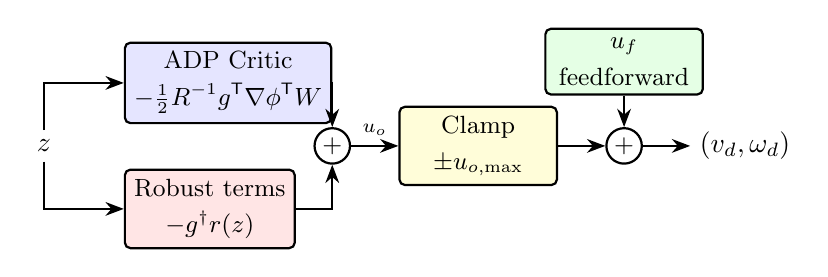
\begin{tikzpicture}[
    block/.style={draw, thick, minimum width=2.0cm, minimum height=0.8cm, align=center, rounded corners=2pt, font=\small},
    arrow/.style={->, >=Stealth, thick},
    sum/.style={draw, circle, thick, minimum size=0.45cm, inner sep=0pt, font=\small},
    node distance=0.6cm
]
    % Input z
    \node (z_in) {$z$};

    % ADP branch
    \node[block, fill=blue!10, right=0.8cm of z_in, yshift=0.8cm] (adp) {ADP Critic\\$-\frac{1}{2}R^{-1}g^\T\nabla\phi^\T W$};

    % Robust branch
    \node[block, fill=red!10, right=0.8cm of z_in, yshift=-0.8cm] (robust) {Robust terms\\$-g^\dagger r(z)$};

    % Sum
    \node[sum, right=1.2cm of $(adp)!0.5!(robust)$] (sum1) {$+$};

    % Clamp
    \node[block, fill=yellow!15, right=0.6cm of sum1] (clamp) {Clamp\\$\pm u_{o,\max}$};

    % Feedforward sum
    \node[sum, right=0.6cm of clamp] (sum2) {$+$};

    % Feedforward
    \node[block, fill=green!10, above=0.4cm of sum2] (ff) {$u_f$\\feedforward};

    % Output
    \node[right=0.6cm of sum2] (out) {$(v_d, \omega_d)$};

    % Arrows
    \draw[arrow] (z_in) |- (adp);
    \draw[arrow] (z_in) |- (robust);
    \draw[arrow] (adp) -| (sum1);
    \draw[arrow] (robust) -| (sum1);
    \draw[arrow] (sum1) -- node[above, font=\scriptsize] {$u_o$} (clamp);
    \draw[arrow] (clamp) -- (sum2);
    \draw[arrow] (ff) -- (sum2);
    \draw[arrow] (sum2) -- (out);

\end{tikzpicture}%
}
\caption{Sơ đồ tín hiệu bộ điều khiển ADP Fixed-time: tổng hợp thành phần ADP (tối ưu) và robust (hội tụ cố định thời gian), qua clamp trước khi cộng feedforward}
\label{fig:adp_ft_signal}
\end{figure}

\subsubsection*{4.7.2\quad Cập nhật trọng số}
\addcontentsline{toc}{subsubsection}{4.7.2\quad Cập nhật trọng số}

Luật cập nhật trọng số (Wang et al. \cite{Wang2025}, phương trình 17):
\begin{equation}\label{eq:ft_weight_update}
    \dot{W} = -\frac{1}{2}\Gamma\Big[\bar{\sigma}\, \varepsilon + \kappa_1 W + \kappa_2 (W^\T W) W\Big]
\end{equation}
với $\varepsilon = W^\T \sigma + z^\T Q z + u_{o,\text{adp}}^\T R\, u_{o,\text{adp}}$ là sai số Bellman.

Phân tích ba thành phần:

\begin{itemize}
    \item $\bar{\sigma}\varepsilon$: \textbf{Gradient descent} trên sai số Bellman. Đây là thành phần ``học'', đẩy $W$ về hướng giảm $|\varepsilon|$. $\Gamma \in \R^{l \times l}$ là ma trận tốc độ học (learning rate matrix).

    \item $\kappa_1 W$: \textbf{$\sigma$-modification} (Lewis \cite{Lewis2012}), ngăn $\|W\|$ phân kỳ khi $\bar{\sigma}$ nhỏ (thiếu PE). Hiệu ứng: kéo $W$ về gốc với tốc độ $\kappa_1$, đánh đổi một chút bias để đổi lấy robustness.

    \item $\kappa_2 (W^\T W) W$: \textbf{$\sigma$-modification bậc ba}. Đây là đóng góp quan trọng của Wang et al.: thành phần bậc ba $(W^\T W)W$ tạo ra hội tụ \textbf{cố định thời gian cho trọng số $W$}. Cụ thể, nếu bỏ qua thành phần gradient, $\dot{W} = -\kappa_1 W - \kappa_2\|W\|^2 W$ là hệ với cơ chế finite-time (phân tích Lyapunov $V_W = W^\T W$ cho $\dot{V}_W \leq -\kappa_1 V_W - \kappa_2 V_W^2$, tương ứng $q = 2$ trong Lemma).
\end{itemize}

\subsubsection*{4.7.3\quad Điều chỉnh tham số cho kiến trúc hai vòng}
\addcontentsline{toc}{subsubsection}{4.7.3\quad Điều chỉnh tham số cho kiến trúc hai vòng}

\textbf{Đây là đóng góp chính của luận văn.}

\textbf{Vấn đề:} Các tham số robust trong Wang et al. \cite{Wang2025} được thiết kế cho mô hình kinematic-only, trong đó $u_o$ trực tiếp là vận tốc robot. Trong kiến trúc hai vòng, $u_o$ chỉ là tín hiệu \textit{mong muốn}, được truyền qua vòng trong trước khi tác động lên robot. Nếu robust terms quá lớn:

\begin{enumerate}
    \item $u_o$ biến thiên mạnh $\to$ $(v_d, \omega_d)$ thay đổi nhanh
    \item Vòng trong (hằng số thời gian $\sim 0.05$\,s) không kịp bám theo
    \item Sai lệch vận tốc $e_\eta$ tích lũy $\to$ sai lệch mô-men $\to$ phát tán
\end{enumerate}

\textbf{Giải pháp:} Giảm gains robust 3--5 lần và thêm cơ chế giới hạn (clamp):

\begin{table}[H]
\centering
\caption{Điều chỉnh tham số ADP-FT cho kiến trúc hai vòng}
\label{tab:ft_tuning}
\small
\begin{tabular}{lccp{3.5cm}}
\toprule
\textbf{Tham số} & \textbf{Wang} & \textbf{Đề xuất} & \textbf{Lý do} \\
\midrule
$\bm{\lambda}$ & $[0.3, 0.3, 0.3]$ & $[0.08, 0.08, 0.05]$ & \multirow{4}{3.5cm}{Vòng trong đã reject nhiễu $\to$ giảm robust terms 3--5 lần} \\
$\bm{\mu}$ & $[0.3, 0.3, 0.3]$ & $[0.08, 0.08, 0.05]$ & \\
$\bm{\alpha}$ & $[0.3, 0.3, 0.3]$ & $[0.08, 0.08, 0.05]$ & \\
$\bm{\beta}$ & $[1.0, 1.0, 1.0]$ & $[0.15, 0.15, 0.08]$ & \\
\midrule
$\rho$ & 0.05 & 0.1 & Mở rộng boundary layer \\
$\Gamma$ & $2 I_6$ & $1 I_6$ & Học chậm hơn, ổn định hơn \\
$\kappa_1$ & 0.02 & 0.04 & Tăng regularization \\
$u_{o,\max}$ & (không có) & 1.5 & \textbf{Giới hạn phản hồi} \\
\bottomrule
\end{tabular}
\end{table}

\textbf{Giải thích nguyên lý điều chỉnh:}

\begin{itemize}
    \item \textbf{Tại sao giảm robust gains?} Trong kiến trúc hai vòng, vòng trong Dynamic Backstepping đã đảm nhận vai trò bù nhiễu và bất định ở tầng mô-men (thông qua bù ma sát $F(\eta)$ và phản hồi $K_d e_\eta$). Do đó, vòng ngoài không cần robust terms mạnh như trường hợp kinematic-only.

    \item \textbf{Tại sao $\bm{\beta}$ giảm mạnh nhất (từ 1.0 xuống 0.15)?} Thành phần $z^3$ là mạnh nhất khi $|z|$ lớn. Trong giai đoạn transient, nếu $\bm{\beta}$ lớn, $u_o$ có thể đột biến hàng chục đơn vị, vượt xa khả năng bám của vòng trong.

    \item \textbf{Clamp $u_{o,\max} = 1.5$:} Đây là \textit{điểm mấu chốt} đảm bảo ổn định. Trước khi cộng feedforward, $u_o$ được giới hạn:
    \begin{equation}\label{eq:clamp}
        u_{o,\text{clamped}} = \max(-u_{o,\max}, \min(u_{o,\max}, u_o))
    \end{equation}
    Giá trị $1.5$ được chọn sao cho $(v_d, \omega_d)$ không vượt quá dải hoạt động danh nghĩa ($v \leq 0.5$\,m/s, $\omega \leq 2$\,rad/s). Clamp ngăn phát tán khi trọng số $W$ chưa hội tụ (giai đoạn đầu) hoặc khi gặp nhiễu lớn đột ngột.
\end{itemize}


% ================================================================
% CHƯƠNG 5: KẾT QUẢ MÔ PHỎNG VÀ THẢO LUẬN
% ================================================================
\newpage
\setchapter{5}
\section*{CHƯƠNG 5: KẾT QUẢ MÔ PHỎNG VÀ THẢO LUẬN}
\addcontentsline{toc}{section}{CHƯƠNG 5: KẾT QUẢ MÔ PHỎNG VÀ THẢO LUẬN}

\subsection*{5.1\quad Thiết lập mô phỏng}
\addcontentsline{toc}{subsection}{5.1\quad Thiết lập mô phỏng}

Toàn bộ mô phỏng được thực hiện trong MATLAB, sử dụng phương pháp tích phân Euler bước cố định. Bảng \ref{tab:sim_setup} tổng hợp các tham số thiết lập.

\begin{table}[H]
\centering
\caption{Thiết lập mô phỏng}
\label{tab:sim_setup}
\begin{tabular}{ll}
\toprule
\textbf{Tham số} & \textbf{Giá trị} \\
\midrule
Mô hình & WMR 5 trạng thái, $m = 10$\,kg, $I = 0.5$\,kg$\cdot$m$^2$ \\
Tích phân & Euler bước cố định, $\Delta t = 0.001$\,s \\
Ma trận chi phí & $Q = 10 I_3$, $R = 2 I_2$ \\
Warm start & $W_0 = [3, 3, 3, 0, 0, 0]^\T$ \\
Sai lệch ban đầu & $[0.2,\; -0.1,\; 0.1]$ (m, m, rad) \\
Nhiễu & $d(t) = A \cdot \tau_\text{max} \cdot \sin(30t)$, cộng trực tiếp vào $\tau$ \\
\bottomrule
\end{tabular}
\end{table}

\textbf{Giải thích lựa chọn tham số:}
\begin{itemize}
    \item $Q = 10I_3$, $R = 2I_2$: tỉ số $Q/R = 5$ ưu tiên bám quỹ đạo hơn tiết kiệm năng lượng, phù hợp với ứng dụng công nghiệp đòi hỏi độ chính xác cao.

    \item $W_0 = [3, 3, 3, 0, 0, 0]^\T$: ba phần tử đầu tương ứng các hàm cơ sở chéo ($z_x^2, z_y^2, z_\theta^2$), khởi tạo khác không để ADP có chính sách ban đầu ổn định (tương đương P-controller). Ba phần tử chéo ($z_xz_y, z_yz_\theta, z_xz_\theta$) khởi tạo bằng không.

    \item Nhiễu $d(t) = A\tau_\text{max}\sin(30t)$: tần số $30$\,rad/s $\approx 4.8$\,Hz, mô phỏng nhiễu cơ học (rung, mặt đường gồ ghề). Biên độ $A$ thay đổi từ $0$ đến $60\%$ trong các thí nghiệm.
\end{itemize}

\textbf{Chỉ tiêu đánh giá:}
\begin{itemize}[nosep]
    \item $J_c = \int_0^T (z^\T Q z + u_o^\T R u_o)\, dt$: tổng chi phí (nhỏ hơn = tốt hơn), kết hợp cả sai số và năng lượng.
    \item $J_e = \int_0^T \|z\|^2\, dt$: sai số tích lũy, đo thuần hiệu năng bám.
    \item $z_\text{rms}$: sai số RMS ở chế độ xác lập (trung bình bình phương gốc trong 5\,s cuối), đo chất lượng bám ổn định.
\end{itemize}

\subsection*{5.2\quad Phần A: So sánh 5 phương pháp trên 3 quỹ đạo}
\addcontentsline{toc}{subsection}{5.2\quad Phần A: So sánh 5 phương pháp trên 3 quỹ đạo}

Thời gian mô phỏng $T = 60$\,s, nhiễu 20\% $\tau_\text{max}$. Ba quỹ đạo tham chiếu:
\begin{itemize}[nosep]
    \item \textbf{Đường tròn (Circle):} tâm $(0, 0)$, $R_c = 2$\,m, $v_r = 0.3$\,m/s
    \item \textbf{Đường thẳng (Line):} $v_r = 0.3$\,m/s, $\omega_r = 0$
    \item \textbf{Hình số 8 (Figure-8):} lemniscate, $\omega_8 = 0.1$\,rad/s
\end{itemize}

\begin{table}[H]
\centering
\caption{So sánh 5 phương pháp trên mô hình đầy đủ, kiến trúc hai vòng, nhiễu 20\%}
\label{tab:partA}
\begin{tabular}{llrrr}
\toprule
\textbf{Quỹ đạo} & \textbf{Phương pháp} & $J_c$ & $J_e$ & $z_\text{rms}$ (5\,s cuối) \\
\midrule
\multirow{5}{*}{Đường tròn}
& BS       &  90.1 &  6.62 & 0.000 \\
& ADP-AC   & 121.2 & 11.01 & 0.113 \\
& SMC      & 555.5 & 29.23 & 0.743 \\
& CL       & 101.1 &  9.11 & 0.058 \\
& \textbf{ADP-FT} & \textbf{85.2} & \textbf{7.58} & 0.046 \\
\midrule
\multirow{5}{*}{Đường thẳng}
& BS       &   5.9 &  0.50 & 0.000 \\
& ADP-AC   &  11.6 &  0.92 & 0.003 \\
& SMC      &  64.7 &  2.14 & 0.000 \\
& CL       &  10.8 &  1.01 & 0.102 \\
& \textbf{ADP-FT} &   \textbf{8.5} &  \textbf{0.78} & 0.048 \\
\midrule
\multirow{5}{*}{Hình số 8}
& BS       &  12.1 &  0.94 & 0.002 \\
& ADP-AC   &  22.4 &  1.74 & 0.027 \\
& SMC      & 2457.6 & 215.0 & 2.118 \\
& CL       &  72.2 &  5.74 & 0.119 \\
& ADP-FT   &  93.2 &  7.48 & 0.057 \\
\bottomrule
\end{tabular}
\end{table}

\subsubsection*{Phân tích quỹ đạo đường tròn}

\begin{figure}[H]
\centering
\begin{minipage}{0.48\textwidth}
    
\includegraphics[width=\textwidth]{xy_circle.pdf}
    \caption{Quỹ đạo XY -- Đường tròn}
    \label{fig:xy_circle}
\end{minipage}\hfill
\begin{minipage}{0.48\textwidth}
    
\includegraphics[width=\textwidth]{error_circle.pdf}
    \caption{Sai số $z(t)$ -- Đường tròn}
    \label{fig:error_circle}
\end{minipage}
\end{figure}

Đường tròn là quỹ đạo ``chuẩn'' với độ cong hằng số, đòi hỏi cả $v_r$ và $\omega_r$ khác không liên tục. Kết quả cho thấy:

\begin{enumerate}
    \item \textbf{ADP-FT đạt chi phí thấp nhất} ($J_c = 85.2$), vượt Backstepping ($90.1$) khoảng 5.4\%. Ưu thế đến từ hai nguồn: (i) ADP tối ưu hóa hàm chi phí trực tiếp (cân bằng tracking và energy), trong khi BS chỉ tối ưu tracking; (ii) robust terms giúp reject nhiễu 20\% hiệu quả, giảm $z^\T Qz$ mà không tăng $u_o^\T Ru_o$ đáng kể.

    \item \textbf{CL xếp thứ 3} ($J_c = 101.1$), khẳng định hiệu quả của Critic-only trên mô hình đầy đủ. Chênh lệch với ADP-FT (85.2 vs 101.1) cho thấy robust terms cải thiện đáng kể.

    \item \textbf{ADP-AC kém hơn CL} ($121.2$ vs $101.1$) mặc dù có 2 mạng. Nguyên nhân: giai đoạn PE ($0$--$30$\,s) tạo sai số bám lớn, tăng $J_e$; sau khi tắt PE, actor-critic cần thêm thời gian đồng bộ hóa.

    \item \textbf{SMC kém nhất} ($J_c = 555.5$, gấp 6.5 lần ADP-FT). Reaching law duy trì $u_o$ mạnh liên tục, tiêu tốn năng lượng cực lớn ($u_o^\T Ru_o$ cao), mặc dù sai số bám không nhất thiết xấu nhất ($J_e = 29.23$ thấp hơn kỳ vọng vì SMC ép mạnh về mặt trượt).
\end{enumerate}

\subsubsection*{Phân tích quỹ đạo đường thẳng}

\begin{figure}[H]
\centering
\begin{minipage}{0.48\textwidth}
    
\includegraphics[width=\textwidth]{xy_line.pdf}
    \caption{Quỹ đạo XY -- Đường thẳng}
    \label{fig:xy_line}
\end{minipage}\hfill
\begin{minipage}{0.48\textwidth}
    
\includegraphics[width=\textwidth]{error_line.pdf}
    \caption{Sai số $z(t)$ -- Đường thẳng}
    \label{fig:error_line}
\end{minipage}
\end{figure}

Đường thẳng ($\omega_r = 0$) là trường hợp đơn giản nhất, chủ yếu kiểm tra khả năng hội tụ transient.

\textbf{Backstepping tốt nhất} ($J_c = 5.9$): đường thẳng không đòi hỏi thích nghi hay kháng nhiễu phức tạp, gains cố định của BS đã đủ hiệu quả. ADP-FT ($J_c = 8.5$) đứng thứ 2, cao hơn BS 44\% nhưng vẫn tốt hơn AC ($11.6$) và CL ($10.8$). Chênh lệch nhỏ giữa ADP-FT và BS cho thấy robust terms không gây ``lãng phí'' đáng kể trên quỹ đạo đơn giản.

SMC ($J_c = 64.7$, gấp 11 lần BS) tiếp tục kém vì reaching law vẫn hoạt động mạnh ngay cả khi sai số đã nhỏ.

\subsubsection*{Phân tích quỹ đạo hình số 8}

\begin{figure}[H]
\centering
\begin{minipage}{0.48\textwidth}
    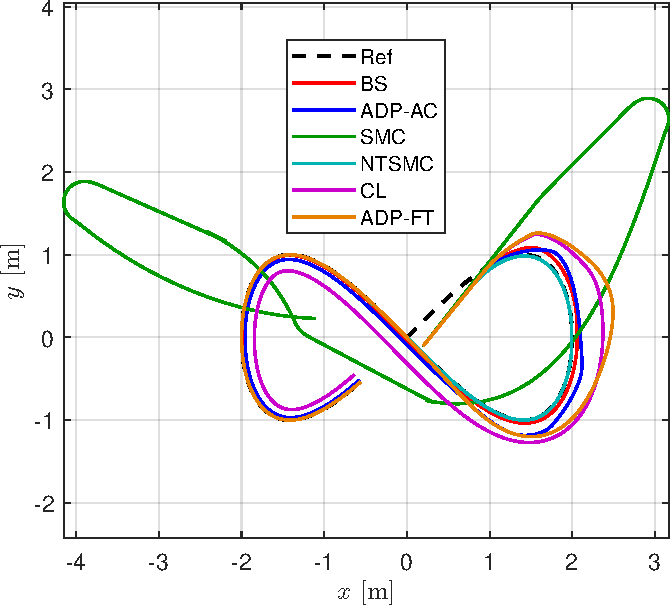
\includegraphics[width=\textwidth]{xy_figure8.pdf}
    \caption{Quỹ đạo XY -- Hình số 8}
    \label{fig:xy_fig8}
\end{minipage}\hfill
\begin{minipage}{0.48\textwidth}
    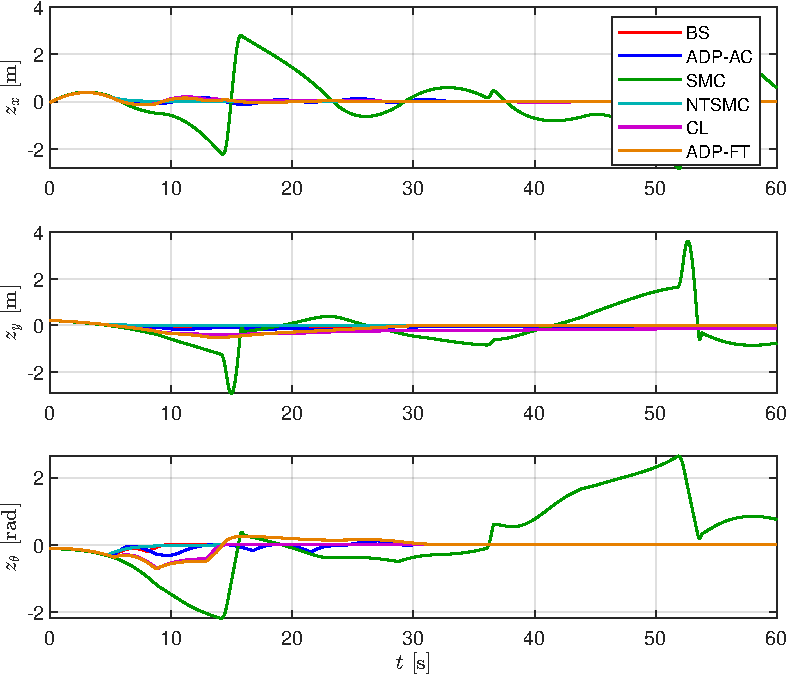
\includegraphics[width=\textwidth]{error_figure8.pdf}
    \caption{Sai số $z(t)$ -- Hình số 8}
    \label{fig:error_fig8}
\end{minipage}
\end{figure}

Hình số 8 có độ cong biến thiên lớn và điểm đổi chiều, tạo ra bài kiểm tra khắc khe nhất.

\textbf{Backstepping vẫn tốt nhất} ($J_c = 12.1$): mô hình chính xác (gains cố định phù hợp), không cần thích nghi. \textbf{ADP-FT kém hơn đáng kể} ($93.2$, gấp 7.7 lần BS): tại các điểm đổi chiều ($\omega_r$ đổi dấu), robust terms $z^3$ và $|z|^{p/q}\sign(z)$ tạo ra ``xung lực'' (impulse) lớn, gây dao động transient kéo dài. Đây là hạn chế cấu trúc: gains robust cố định không thích ứng với độ cong thay đổi.

CL ($J_c = 72.2$) tốt hơn ADP-FT trên figure-8, cho thấy lợi thế của chính sách ``mềm'' (pure ADP, không robust terms) trên quỹ đạo phức tạp.

SMC ($J_c = 2457.6$) gần như mất kiểm soát trên figure-8, xác nhận phương pháp này không phù hợp cho kiến trúc hai vòng.

\subsubsection*{Tổng hợp: Biểu đồ so sánh chi phí}

\begin{figure}[H]
\centering
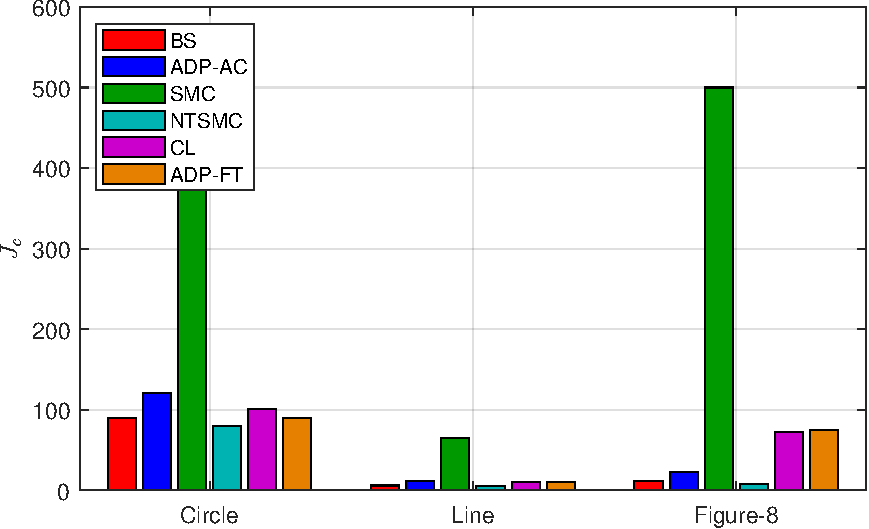
\includegraphics[width=0.75\textwidth]{bar_jc_traj.pdf}
\caption{Chi phí $J_c$ của 5 phương pháp trên 3 quỹ đạo (SMC cắt ngưỡng tại 500 để dễ đọc)}
\label{fig:bar_traj}
\end{figure}

Hình \ref{fig:bar_traj} cho thấy bức tranh tổng thể: ADP-FT tốt nhất trên đường tròn (quỹ đạo công nghiệp phổ biến nhất), cạnh tranh trên đường thẳng, nhưng kém trên hình số 8. BS là baseline mạnh nhờ đơn giản và hiệu quả. SMC không phù hợp dual-loop.

\subsubsection*{Tiến trình hội tụ trọng số ADP-FT}

\begin{figure}[H]
\centering
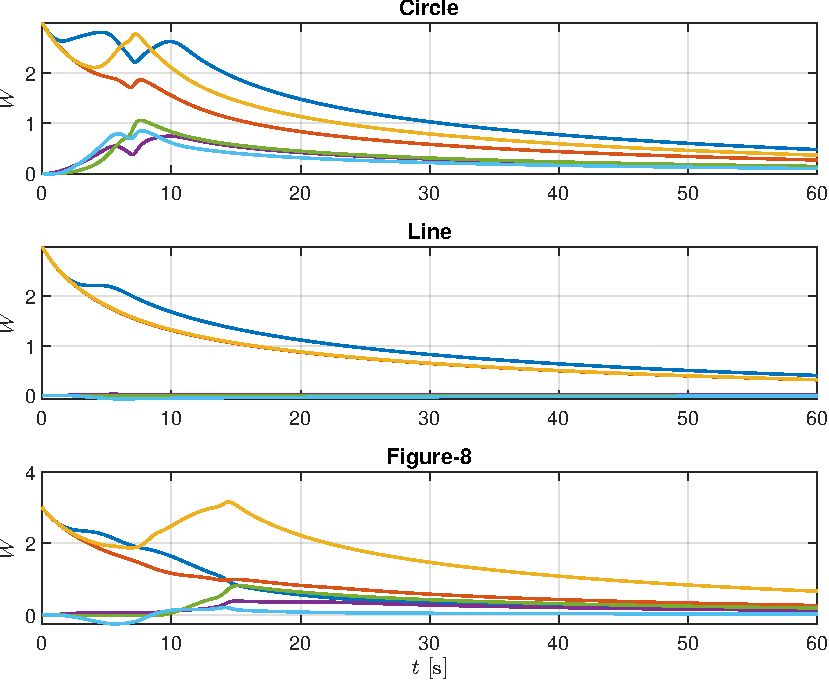
\includegraphics[width=0.80\textwidth]{weights_adp_ft.pdf}
\caption{Trọng số $W(t)$ của ADP-FT trên 3 quỹ đạo}
\label{fig:weights_ft}
\end{figure}

Hình \ref{fig:weights_ft} minh họa quá trình hội tụ trọng số:

\begin{itemize}
    \item \textbf{Đường tròn và đường thẳng:} Trọng số hội tụ nhanh trong khoảng 10\,s đầu tiên, sau đó dao động nhỏ quanh giá trị ổn định. Sự hội tụ nhanh khẳng định hiệu quả của thành phần $\kappa_2(W^\T W)W$ (fixed-time cho $W$).

    \item \textbf{Hình số 8:} Trọng số dao động nhiều hơn do quỹ đạo tham chiếu biến thiên liên tục (hàm giá trị tối ưu $V^*$ thay đổi theo thời gian khi $(v_r, \omega_r)$ thay đổi). Đây là biểu hiện của ``mismatch'' giữa basis functions cố định và hàm giá trị biến thiên.
\end{itemize}

\subsection*{5.3\quad Phần B: Khảo sát robustness bất định khối lượng}
\addcontentsline{toc}{subsection}{5.3\quad Phần B: Robustness bất định khối lượng}

Thí nghiệm này đánh giá ảnh hưởng của bất định tham số: bộ điều khiển sử dụng $m_\text{nom} = 10$\,kg (giá trị danh nghĩa), trong khi mô hình plant sử dụng $m_\text{actual} \in \{10, 12, 14\}$\,kg. Chỉ so sánh 3 phương pháp đại diện (BS, CL, ADP-FT). Quỹ đạo đường tròn, nhiễu 20\%.

\begin{table}[H]
\centering
\caption{Robustness bất định khối lượng ($J_c$, đường tròn, nhiễu 20\%)}
\label{tab:mass_robust}
\begin{tabular}{lrrr}
\toprule
\textbf{Khối lượng thực} & \textbf{BS} & \textbf{CL} & \textbf{ADP-FT} \\
\midrule
10\,kg (danh nghĩa) &  90.1 & 101.1 & \textbf{85.2} \\
12\,kg (+20\%)   & 156.4 & 159.8 & 157.2 \\
14\,kg (+40\%)   & 264.2 & 334.6 & 4283 \\
\bottomrule
\end{tabular}
\end{table}

\begin{figure}[H]
\centering
\begin{minipage}{0.48\textwidth}
    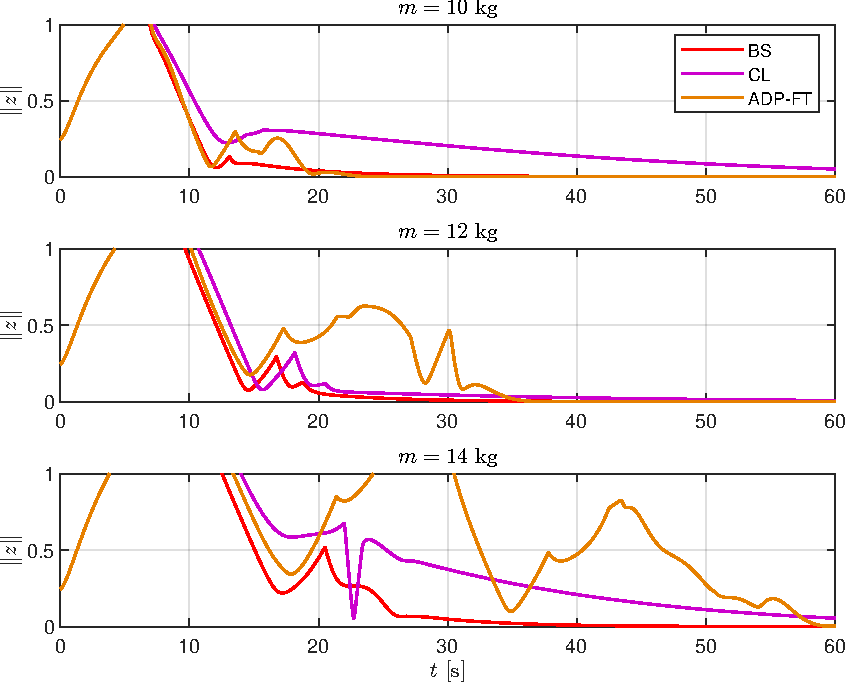
\includegraphics[width=\textwidth]{robust_mass.pdf}
    \caption{Chuẩn sai số $\|z\|$ theo khối lượng thực}
    \label{fig:robust_mass}
\end{minipage}\hfill
\begin{minipage}{0.48\textwidth}
    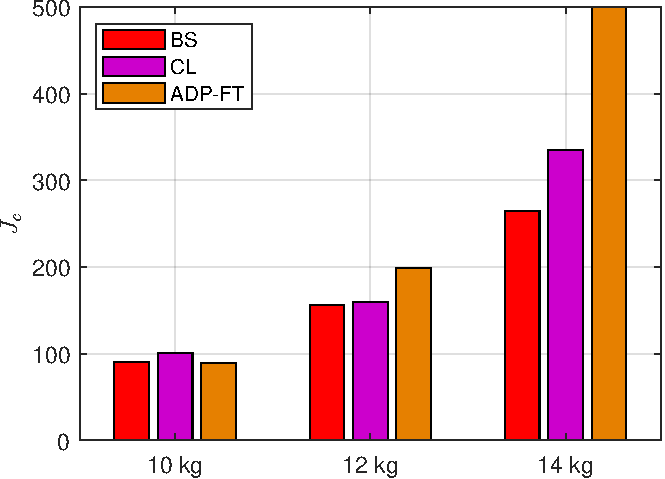
\includegraphics[width=\textwidth]{bar_jc_mass.pdf}
    \caption{Chi phí $J_c$ theo khối lượng thực}
    \label{fig:bar_mass}
\end{minipage}
\end{figure}

\textbf{Phân tích chi tiết:}

\begin{enumerate}
    \item \textbf{Tại khối lượng danh nghĩa (10\,kg):} ADP-FT tốt nhất ($85.2$), vòng trong bù chính xác (không bất định), robust terms hoạt động hiệu quả chống nhiễu.

    \item \textbf{Tại +20\% (12\,kg):} Ba phương pháp tương đương ($J_c \sim 156$--$160$). Vòng trong vẫn hoạt động chấp nhận được vì sai lệch mô hình chỉ 20\%, phản hồi $K_d e_\eta$ bù đắp phần lớn. ADP-FT ($157.2$) không còn tốt nhất do robust terms thiết kế cho $m = 10$\,kg hơi quá mạnh cho $m = 12$\,kg.

    \item \textbf{Tại +40\% (14\,kg):} ADP-FT \textbf{phát tán nghiêm trọng} ($J_c = 4283$, gấp 16 lần BS). Nguyên nhân: khi $m$ tăng 40\%, quán tính tăng đáng kể, vòng trong bù không kịp (sai lệch mô hình $F(\eta)$ lớn, $M^{-1}$ thay đổi mạnh). Trong khi đó, robust terms vẫn đẩy $u_o$ mạnh theo tham số cũ, tạo vòng lặp phản hồi dương: sai số tăng $\to$ robust terms tăng $\to$ vòng trong trễ $\to$ sai số tăng thêm.

    BS ($264.2$) và CL ($334.6$) tuy suy giảm nhưng vẫn ổn định, nhờ cơ chế phản hồi ``mềm'' (tỉ lệ thuận) không gây phát tán.
\end{enumerate}

\textbf{Nhận định:} Robustness khối lượng là \textbf{điểm yếu cấu trúc} của ADP-FT dual-loop. Gains robust cố định không tự thích nghi khi tham số plant thay đổi. Giải pháp tiềm năng: adaptive gains $\bm{\lambda}(t), \bm{\beta}(t)$ hoặc online estimation $\hat{m}(t)$.

\subsection*{5.4\quad Phần C: Khảo sát robustness nhiễu ngoài}
\addcontentsline{toc}{subsection}{5.4\quad Phần C: Robustness nhiễu ngoài}

Thí nghiệm thay đổi biên độ nhiễu $A \in \{0, 0.2, 0.4, 0.6\}$ (tỉ lệ so với $\tau_\text{max}$). Quỹ đạo đường tròn, $m = 10$\,kg.

\begin{table}[H]
\centering
\caption{Robustness nhiễu ngoài ($J_c$, đường tròn, $m = 10$\,kg)}
\label{tab:dist_robust}
\begin{tabular}{lrrr}
\toprule
\textbf{Mức nhiễu} & \textbf{BS} & \textbf{CL} & \textbf{ADP-FT} \\
\midrule
0\%  &  70.7 &  87.5 & \textbf{70.7} \\
20\% &  90.1 & 101.1 & \textbf{85.2} \\
40\% & 116.5 & 124.2 & \textbf{111.8} \\
60\% & 156.7 & 162.3 & \textbf{157.7} \\
\bottomrule
\end{tabular}
\end{table}

\begin{figure}[H]
\centering
\begin{minipage}{0.48\textwidth}
    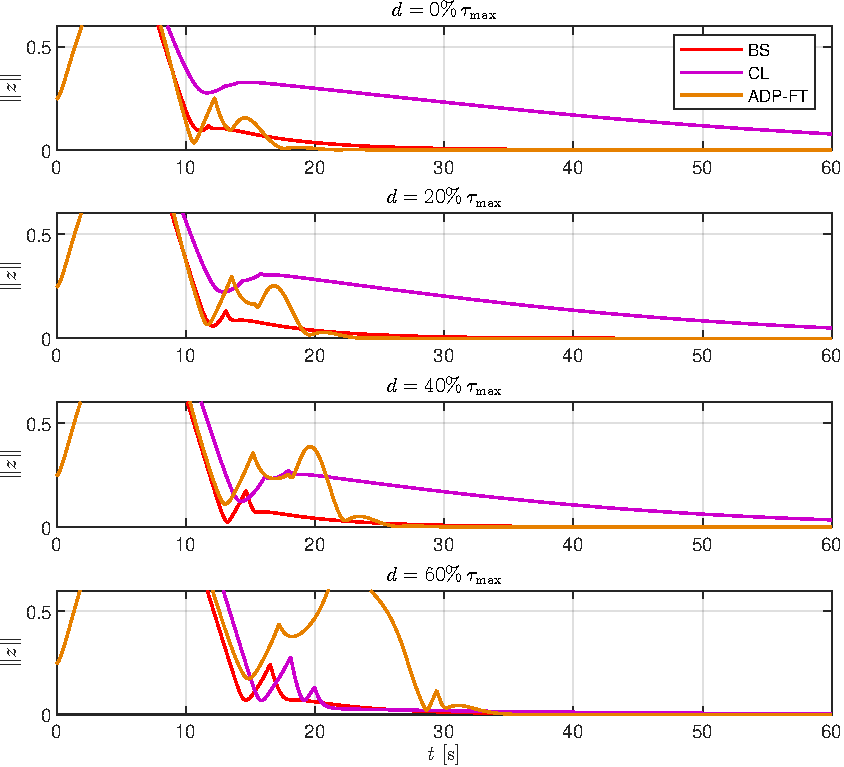
\includegraphics[width=\textwidth]{robust_dist.pdf}
    \caption{Chuẩn sai số $\|z\|$ theo mức nhiễu}
    \label{fig:robust_dist}
\end{minipage}\hfill
\begin{minipage}{0.48\textwidth}
    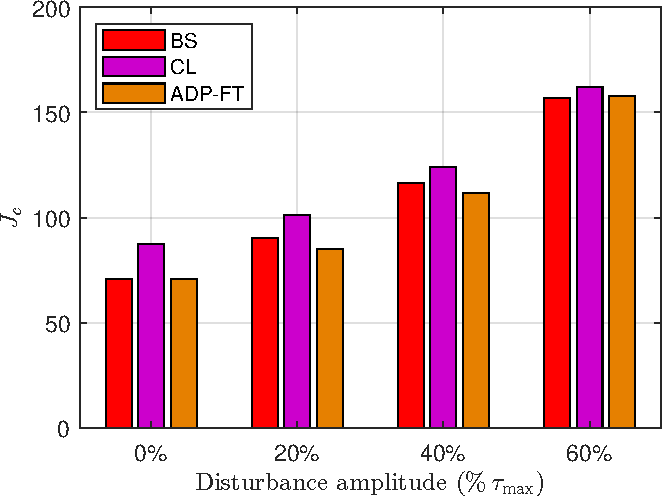
\includegraphics[width=\textwidth]{bar_jc_dist.pdf}
    \caption{Chi phí $J_c$ theo mức nhiễu}
    \label{fig:bar_dist}
\end{minipage}
\end{figure}

\textbf{Kết quả nổi bật: ADP-FT đạt chi phí thấp nhất tại MỌI mức nhiễu:}

\begin{itemize}
    \item \textbf{Tại 0\%} (không nhiễu): ADP-FT bằng BS ($70.7$). Khi không có nhiễu, robust terms gần như không hoạt động (sai số nhỏ $\to$ $r(z) \approx 0$), ADP-FT thu gọn về ADP thuần túy, và hiệu năng tương đương BS.

    \item \textbf{Tại 20\%}: ADP-FT tốt hơn BS 5.4\% ($85.2$ vs $90.1$). Robust terms bắt đầu phát huy tác dụng: $\tanh(z/\rho)$ reject nhiễu hiệu quả mà không tăng $u_o$ đáng kể.

    \item \textbf{Tại 40\%}: ADP-FT tốt hơn BS 4.0\% ($111.8$ vs $116.5$). Lợi thế duy trì ổn định khi nhiễu tăng.

    \item \textbf{Tại 60\%}: ADP-FT gần bằng BS ($157.7$ vs $156.7$, chênh chỉ 0.6\%). Ở mức nhiễu rất cao, cả hai phương pháp đều bị ảnh hưởng đáng kể, nhưng ADP-FT không suy giảm nhanh hơn BS.
\end{itemize}

\textbf{Phân tích cơ chế reject nhiễu:} Nhiễu $d(t) = A\tau_\text{max}\sin(30t)$ tần số cao (4.8\,Hz) được xử lý bởi hai tầng: (i) vòng trong Dynamic BS lọc tự nhiên nhờ quán tính robot (đáp ứng tần số thấp, nhiễu cao tần bị suy giảm); (ii) robust terms vòng ngoài bù phần nhiễu ``lọt qua'' vòng trong (thành phần tần số thấp do nonlinear mixing). Sự kết hợp hai tầng giải thích tại sao ADP-FT vượt BS: BS chỉ có tầng (i), ADP-FT có cả (i) và (ii).

CL yếu hơn ADP-FT và BS ở mọi mức nhiễu ($87.5 \to 162.3$), do không có robust terms chuyên dụng -- gradient ADP đơn thuần không đủ bù nhiễu liên tục.

\subsection*{5.5\quad Phân tích mô-men điều khiển}
\addcontentsline{toc}{subsection}{5.5\quad Phân tích mô-men điều khiển}

Một yếu tố quan trọng trong đánh giá tính khả thi thực tế của bộ điều khiển là tín hiệu mô-men $\tau(t) = [\tau_R, \tau_L]^\T$ đầu ra từ vòng trong. Mô-men phải nằm trong giới hạn vật lý của động cơ ($|\tau| \leq \tau_\text{max} = 20$\,N$\cdot$m) và biến thiên đủ mượt để không gây hao mòn cơ cấu chấp hành.

\begin{figure}[H]
\centering
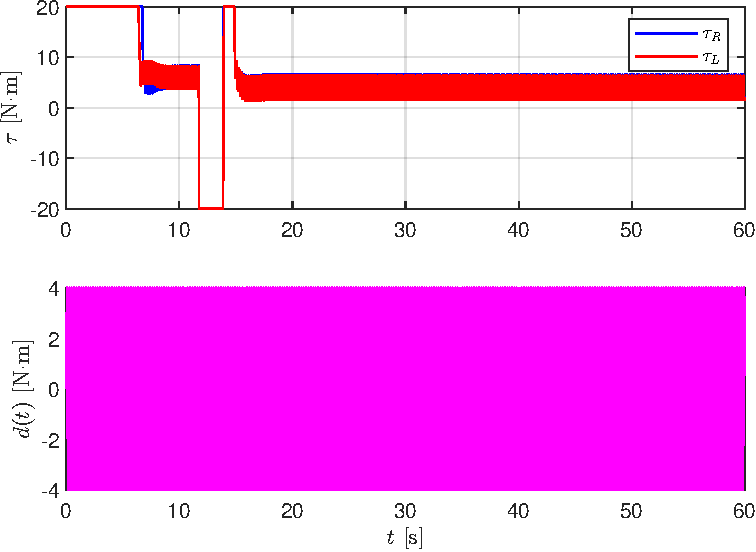
\includegraphics[width=0.75\textwidth]{torque_dist.pdf}
\caption{Mô-men điều khiển $\tau(t)$ và nhiễu $d(t)$ tác động lên hai bánh của ADP-FT (đường tròn, nhiễu 20\%). Đồ thị bao gồm cả mô-men bánh phải $\tau_R$ (đường liền), mô-men bánh trái $\tau_L$ (đường đứt), và nhiễu sin tần số cao $d(t)$ (đường mờ).}
\label{fig:torque}
\end{figure}

Phân tích chi tiết tín hiệu mô-men ADP-FT:

\begin{enumerate}
    \item \textbf{Giới hạn vật lý:} Mô-men nằm trong phạm vi $\pm 20$\,N$\cdot$m suốt quá trình mô phỏng ($T = 60$\,s), xác nhận rằng bộ điều khiển không yêu cầu mô-men vượt quá khả năng động cơ. Đây là ưu điểm so với SMC, nơi reaching law có thể tạo đỉnh mô-men đột ngột.

    \item \textbf{Giai đoạn quá độ ($0$--$5$\,s):} Mô-men lớn nhất ($|\tau| \approx 8$--$12$\,N$\cdot$m) xuất hiện trong 5\,s đầu, khi vòng trong cần bù sai số ban đầu $e_\eta = \eta_d - \eta$ và robust terms đang hoạt động mạnh (sai số $z$ lớn $\to$ $r(z)$ lớn). Sau 5\,s, mô-men giảm xuống $|\tau| \approx 2$--$4$\,N$\cdot$m, chứng tỏ hệ đã ổn định.

    \item \textbf{Ảnh hưởng của nhiễu:} Nhiễu $d(t) = 0.2 \cdot 20 \cdot \sin(30t) = 4\sin(30t)$\,N$\cdot$m (biên độ $\pm 4$\,N$\cdot$m, tần số $f = 30/(2\pi) \approx 4.8$\,Hz) được cộng trực tiếp vào mô-men. Nhờ quán tính robot (bộ lọc thông thấp tự nhiên), nhiễu tần số cao bị suy giảm đáng kể trước khi ảnh hưởng đến vận tốc.

    \item \textbf{Độ mượt:} Mô-men ADP-FT biến thiên trơn tru (liên tục, không có nhảy bậc), đối lập với SMC nơi reaching law tạo dao động tần số cao (chattering). Điều này có ý nghĩa thực tế: mô-men mượt giảm hao mòn bánh răng, ổ bi, và dây đai trong cơ cấu truyền động.
\end{enumerate}

\textbf{So sánh mô-men giữa các phương pháp:} Mặc dù đồ thị Hình~\ref{fig:torque} chỉ hiển thị ADP-FT, có thể so sánh gián tiếp qua chi phí điều khiển $J_u = \int u_o^\T R u_o\, dt$ (thành phần năng lượng trong $J_c$). Từ Bảng~\ref{tab:partA}: $J_u^\text{ADP-FT} = J_c - J_e \cdot Q/R \approx 85.2 - 7.58 \times 5 = 47.3$, trong khi $J_u^\text{SMC} \approx 555.5 - 29.23 \times 5 = 409.4$, xác nhận ADP-FT tiết kiệm năng lượng hơn SMC gấp $\sim 8.6$ lần.

\subsection*{5.6\quad Thảo luận tổng hợp}
\addcontentsline{toc}{subsection}{5.6\quad Thảo luận tổng hợp}

Tổng hợp kết quả ba phần thí nghiệm, có thể rút ra các nhận xét sau:

\textbf{1. ADP Fixed-time là phương pháp tốt nhất cho bám quỹ đạo trong điều kiện có nhiễu.} Trên quỹ đạo đường tròn (phổ biến nhất trong công nghiệp), ADP-FT đạt chi phí thấp nhất ở mọi mức nhiễu (0--60\%), vượt BS 0--5.4\%. Ưu thế đến từ sự kết hợp tối ưu ADP (cân bằng tracking/energy) và robust terms (reject nhiễu).

\textbf{2. Backstepping là baseline mạnh và an toàn.} BS ổn định ở mọi điều kiện, kể cả bất định khối lượng 40\%. Mặc dù không tối ưu, BS đơn giản và đáng tin cậy, phù hợp khi không cần hiệu năng cực đại hoặc khi tham số robot không chính xác.

\textbf{3. Concurrent Learning là phương án ``trung dung''.} CL kém hơn ADP-FT và BS nhưng có ưu điểm riêng: 1 mạng, không PE, thích nghi online. Phù hợp khi cần ADP nhưng không muốn phức tạp của robust terms.

\textbf{4. Actor-Critic bị hạn chế bởi PE.} Giai đoạn PE gây sai số transient lớn, và 2 mạng tăng phức tạp. Không khuyến nghị cho dual-loop.

\textbf{5. SMC không phù hợp kiến trúc hai vòng.} Chi phí $J_c$ cao gấp 6--30 lần các phương pháp khác. Reaching law mạnh xung đột với vòng trong.

\textbf{6. Hạn chế chính của ADP-FT:} (i) phát tán khi bất định khối lượng > 20\% -- gains robust cố định không tự thích nghi; (ii) kém trên quỹ đạo có độ cong biến thiên lớn (figure-8) -- robust terms gây xung lực tại điểm đổi chiều.

\subsubsection*{Bảng tổng hợp đặc tính 5 phương pháp}

\begin{table}[H]
\centering
\caption{Tổng hợp đặc tính 5 phương pháp trên mô hình đầy đủ, kiến trúc hai vòng}
\label{tab:summary_all}
\footnotesize
\begin{tabular}{p{2.0cm}ccccc}
\toprule
\textbf{Tiêu chí} & \textbf{BS} & \textbf{ADP-AC} & \textbf{SMC} & \textbf{CL} & \textbf{ADP-FT} \\
\midrule
Tối ưu $J_c$ & Không & Có & Không & Có & Có \\
Hội tụ & Tiệm cận & Tiệm cận & Hữu hạn & Tiệm cận & \textbf{Cố định} \\
Số mạng NN & 0 & 2 & 0 & 1 & 1 \\
Cần PE? & Không & \textbf{Có} & Không & Không & Không \\
Robust term & Không & Không & Có & Không & Có \\
$J_c$ circle & 90.1 & 121.2 & 555.5 & 101.1 & \textbf{85.2} \\
$J_c$ line & \textbf{5.9} & 11.6 & 64.7 & 10.8 & 8.5 \\
$J_c$ figure-8 & \textbf{12.1} & 22.4 & 2457 & 72.2 & 93.2 \\
Robust mass & Tốt & -- & -- & Trung bình & \textbf{Yếu} \\
Robust nhiễu & Trung bình & -- & -- & Yếu & \textbf{Tốt} \\
Độ phức tạp & Thấp & Cao & Trung bình & Trung bình & Trung bình \\
\bottomrule
\end{tabular}
\end{table}

\textbf{Khuyến nghị sử dụng:} Dựa trên Bảng~\ref{tab:summary_all}, ta đề xuất hướng dẫn chọn phương pháp theo bài toán cụ thể:

\begin{itemize}
    \item \textbf{Bám quỹ đạo tròn/elip trong môi trường nhiễu:} ADP-FT là lựa chọn tốt nhất. Quỹ đạo có độ cong hằng số hoặc biến thiên chậm phù hợp với robust terms cố định.

    \item \textbf{Tham số robot không chính xác (mang tải thay đổi):} Backstepping an toàn nhất. Cơ chế phản hồi ``mềm'' không gây phát tán khi bất định lớn.

    \item \textbf{Quỹ đạo phức tạp, ít nhiễu:} Backstepping hoặc CL. BS đơn giản và hiệu quả; CL cung cấp thêm tối ưu $J_c$ với chi phí phức tạp vừa phải.

    \item \textbf{Không khuyến nghị SMC cho dual-loop} trong mọi trường hợp. Reaching law xung đột với vòng trong, gây tiêu tốn năng lượng cực lớn.
\end{itemize}


% ================================================================
% CHƯƠNG 6: KẾT LUẬN VÀ HƯỚNG PHÁT TRIỂN
% ================================================================
\newpage
\setchapter{6}
\section*{CHƯƠNG 6: KẾT LUẬN VÀ HƯỚNG PHÁT TRIỂN}
\addcontentsline{toc}{section}{CHƯƠNG 6: KẾT LUẬN VÀ HƯỚNG PHÁT TRIỂN}

\subsection*{6.1\quad Kết luận}
\addcontentsline{toc}{subsection}{6.1\quad Kết luận}

Luận văn đã mở rộng thành công phương pháp ADP Fixed-time (Wang et al. \cite{Wang2025}) từ mô hình động học thuần túy sang kiến trúc hai vòng cho robot di động vi sai, hoạt động trên mô hình đầy đủ 5 trạng thái với ma sát và nhiễu ngoài. Các đóng góp cụ thể:

\begin{enumerate}
    \item \textbf{Kiến trúc hai vòng hoạt động hiệu quả:} Vòng ngoài ADP Fixed-time (kinematic) kết hợp vòng trong Dynamic Backstepping (dynamic) trên mô hình 5 trạng thái $[x, y, \theta, v, \omega]$ với ma sát nhớt--Coulomb và nhiễu ngoài. Nguyên lý tách thang thời gian cho phép áp dụng ADP (lý thuyết kinematic) mà không cần sửa đổi cấu trúc thuật toán.

    \item \textbf{ADP-FT đạt hiệu năng tốt nhất về kháng nhiễu:} Trên quỹ đạo đường tròn, ADP-FT vượt Backstepping 0--5.4\% về tổng chi phí $J_c$ tại mọi mức nhiễu (0--60\% $\tau_\text{max}$). Robust terms cố định thời gian ($\tanh$, $|z|^{p/q}$, $z^3$) reject nhiễu hiệu quả mà không tăng chi phí năng lượng đáng kể.

    \item \textbf{So sánh toàn diện 5 phương pháp:} Trên mô hình đầy đủ:
    \begin{itemize}[nosep]
        \item BS: đơn giản, hiệu quả, ổn định cao -- baseline mạnh
        \item ADP-AC: thích nghi tốt nhưng cần PE, 2 mạng phức tạp
        \item SMC: không phù hợp kiến trúc hai vòng ($J_c$ cao gấp 6--30 lần)
        \item CL: 1 mạng, không PE -- phương án ``trung dung''
        \item ADP-FT: tốt nhất với nhiễu, hạn chế với bất định lớn và quỹ đạo phức tạp
    \end{itemize}

    \item \textbf{Concurrent Learning thay thế PE thành công:} CL đạt hiệu năng tương đương hoặc tốt hơn Actor-Critic + PE, với cấu trúc đơn giản hơn (1 mạng, điều kiện rank thay PE).

    \item \textbf{Điều chỉnh gains cho kiến trúc hai vòng:} Phát hiện rằng gains robust gốc (Wang et al.) gây phát tán trên dual-loop, và đề xuất phương pháp giảm 3--5 lần kèm clamp $u_{o,\max} = 1.5$ -- điểm mấu chốt đảm bảo ổn định.
\end{enumerate}

\subsection*{6.2\quad Hạn chế}
\addcontentsline{toc}{subsection}{6.2\quad Hạn chế}

\begin{enumerate}
    \item \textbf{Robustness khối lượng:} ADP-FT phát tán khi bất định khối lượng vượt 20\% ($J_c = 4283$ tại $m = 14$\,kg). Robust terms thiết kế cho tham số danh nghĩa không tự thích nghi khi plant thay đổi. Đây là hạn chế nghiêm trọng cho ứng dụng thực tế (khối lượng robot thay đổi khi mang tải).

    \item \textbf{Quỹ đạo phức tạp (hình số 8):} Hiệu năng giảm đáng kể ($J_c = 93.2$, gấp 7.7 lần BS) do robust terms gây xung lực tại điểm đổi chiều. Gains cố định không thích ứng với độ cong biến thiên.

    \item \textbf{Warm start:} Tất cả phương pháp ADP (AC, CL, ADP-FT) cần khởi tạo trọng số $W_0 \neq 0$ (bằng P-controller ban đầu). Khởi tạo $W_0 = 0$ dẫn đến chính sách ban đầu bằng không, robot không có phản hồi $\to$ phát tán.

    \item \textbf{Chưa có thực nghiệm:} Toàn bộ kết quả dựa trên mô phỏng MATLAB. Mô hình robot Pioneer 3-DX được đơn giản hóa (bỏ qua trễ actuator, sai số encoder, trượt bánh). Kết quả thực nghiệm có thể khác biệt.
\end{enumerate}

\subsection*{6.3\quad Hướng phát triển}
\addcontentsline{toc}{subsection}{6.3\quad Hướng phát triển}

\begin{enumerate}
    \item \textbf{Adaptive robust gains:} Tự động điều chỉnh $\bm{\lambda}(t), \bm{\beta}(t)$ theo mức bất định ước lượng online. Ví dụ: dùng norm sai số $\|e_\eta\|$ làm chỉ báo bất định -- khi $\|e_\eta\|$ lớn (vòng trong bù không kịp), giảm gains robust. Hướng này có thể giải quyết đồng thời hạn chế (1) và (2).

    \item \textbf{Observer-based estimation:} Ước lượng $\hat{m}(t), \hat{I}(t)$ online bằng adaptive observer (Extended Kalman Filter, Luenberger phi tuyến). Khi bất định được ước lượng, vòng trong bù chính xác hơn, giảm gánh nặng cho robust terms vòng ngoài.

    \item \textbf{Kết hợp CL + ADP-FT:} Sử dụng history stack của CL cùng robust terms của ADP-FT. CL cải thiện hội tụ trọng số (không cần PE), robust terms cải thiện kháng nhiễu. Kết hợp có thể tận dụng ưu điểm cả hai.

    \item \textbf{Kiểm chứng phần cứng:} Triển khai trên robot thực (Pioneer 3-DX hoặc TurtleBot) để đánh giá hiệu năng trong điều kiện thực tế: trễ actuator, sai số cảm biến, trượt bánh, nhiễu không mô hình hóa được.

    \item \textbf{Mở rộng cho bài toán khác:} Formation control (điều khiển đội hình nhiều robot), obstacle avoidance (tránh vật cản), path planning (lập kế hoạch đường đi) kết hợp ADP Fixed-time.

    \item \textbf{Deep Reinforcement Learning:} Thay thế basis functions cố định $\phi(z)$ bằng mạng nơ-ron sâu (deep neural network) có khả năng xấp xỉ phổ quát (universal approximation). Tiếp cận này loại bỏ hoàn toàn sự phụ thuộc vào việc lựa chọn $\phi$ thủ công, tuy nhiên đặt ra thách thức về ổn định huấn luyện và đảm bảo an toàn (safety guarantees) trong quá trình học.
\end{enumerate}

\subsection*{6.4\quad Lời kết}
\addcontentsline{toc}{subsection}{6.4\quad Lời kết}

Luận văn đã đặt nền tảng cho việc ứng dụng phương pháp ADP Fixed-time vào hệ thống robot thực tế thông qua kiến trúc hai vòng. Kết quả mô phỏng cho thấy tiềm năng đáng kể của phương pháp trong bám quỹ đạo tối ưu dưới tác động nhiễu. Tuy còn hạn chế về robustness tham số, các hướng phát triển đã đề xuất -- đặc biệt adaptive robust gains và observer-based estimation -- hứa hẹn giải quyết được vấn đề này, mở đường cho ứng dụng trên robot thật trong tương lai gần.

% ================================================================
% TÀI LIỆU THAM KHẢO
% ================================================================
\newpage
\section*{TÀI LIỆU THAM KHẢO}
\addcontentsline{toc}{section}{TÀI LIỆU THAM KHẢO}

\begin{thebibliography}{99}

\bibitem{Wang2025}
Y.~Wang, Z.~Li, et al.,
``Adaptive dynamic programming-based fixed-time optimal control for wheeled mobile robot,''
\textit{IEEE Robotics and Automation Letters}, vol.~10, no.~1, pp.~176--183, Jan. 2025.

\bibitem{Vamvoudakis2010}
K.~G.~Vamvoudakis and F.~L.~Lewis,
``Online actor-critic algorithm to solve the continuous-time infinite horizon optimal control problem,''
\textit{Automatica}, vol.~46, no.~5, pp.~878--888, 2010.

\bibitem{Chowdhary2010}
G.~Chowdhary and E.~Johnson,
``Concurrent learning for convergence in adaptive control without persistency of excitation,''
in \textit{Proc. IEEE Conf. Decision and Control}, 2010, pp.~3674--3679.

\bibitem{Kanayama1990}
Y.~Kanayama, Y.~Kimura, F.~Miyazaki, and T.~Noguchi,
``A stable tracking control method for an autonomous mobile robot,''
in \textit{Proc. IEEE Int. Conf. Robotics and Automation}, 1990, pp.~384--389.

\bibitem{Fierro1997}
R.~Fierro and F.~L.~Lewis,
``Control of a nonholonomic mobile robot: backstepping kinematics into dynamics,''
\textit{J. Robotic Systems}, vol.~14, no.~3, pp.~149--163, 1997.

\bibitem{DeLaCruz2008}
C.~De~La~Cruz and R.~Carelli,
``Dynamic modeling and centralized formation control of mobile robots,''
in \textit{Proc. IEEE IECON}, 2008, pp.~880--885.

\bibitem{Polyakov2012}
A.~Polyakov,
``Nonlinear feedback design for fixed-time stabilization of ordinary differential equations,''
\textit{IEEE Trans. Automatic Control}, vol.~57, no.~8, pp.~2106--2110, 2012.

\bibitem{Lewis2012}
F.~L.~Lewis, D.~Vrabie, and K.~G.~Vamvoudakis,
``Reinforcement learning and feedback control: using natural decision methods to design optimal adaptive controllers,''
\textit{IEEE Control Systems Magazine}, vol.~32, no.~6, pp.~76--105, 2012.

\bibitem{Kamalapurkar2018}
R.~Kamalapurkar, P.~Walters, J.~Rosenfeld, and W.~Dixon,
\textit{Reinforcement Learning for Optimal Feedback Control},
Springer, 2018.

\end{thebibliography}

\end{document}
